% This must be in the first 5 lines to tell arXiv to use pdfLaTeX, which is strongly recommended.
\pdfoutput=1
% In particular, the hyperref package requires pdfLaTeX in order to break URLs across lines.

\documentclass[11pt]{article}

% Remove the "review" option to generate the final version.
% \usepackage[review]{ACL2023}
\usepackage{ACL2023}

% Standard package includes
\usepackage{times}
\usepackage{latexsym}

% For proper rendering and hyphenation of words containing Latin characters (including in bib files)
\usepackage[T1]{fontenc}
% For Vietnamese characters
% \usepackage[T5]{fontenc}
% See https://www.latex-project.org/help/documentation/encguide.pdf for other character sets

% This assumes your files are encoded as UTF8
\usepackage[utf8]{inputenc}

% This is not strictly necessary, and may be commented out.
% However, it will improve the layout of the manuscript,
% and will typically save some space.
\usepackage{microtype}

% This is also not strictly necessary, and may be commented out.
% However, it will improve the aesthetics of text in
% the typewriter font.
\usepackage{inconsolata}
\usepackage{graphicx}
\usepackage{subfigure}
\usepackage{booktabs} % for professional tables

\usepackage{amsfonts}
\usepackage{stfloats}
\usepackage{ulem}

\usepackage{amsmath}
% Attempt to make hyperref and algorithmic work together better:
\newcommand{\theHalgorithm}{\arabic{algorithm}}
\newcommand{\tabincell}[2]{\begin{tabular}{@{}#1@{}}#2\end{tabular}}
\usepackage{adjustbox}
\usepackage{multirow}
\usepackage{array}
\usepackage{float}
\usepackage{caption}
\usepackage{balance}
\usepackage{flushend}

\usepackage{xurl}

\usepackage{listings}
\usepackage{color}

\definecolor{dkgreen}{rgb}{0,0.6,0}
\definecolor{gray}{rgb}{0.5,0.5,0.5}
\definecolor{mauve}{rgb}{0.58,0,0.82}

\lstset{frame=tb,
  language=Python,
  aboveskip=3mm,
  belowskip=3mm,
  showstringspaces=false,
  columns=flexible,
  basicstyle={\small\ttfamily},
  numbers=none,
  numberstyle=\tiny\color{gray},
  keywordstyle=\color{blue},
  commentstyle=\color{dkgreen},
  stringstyle=\color{mauve},
  breaklines=true,
  breakatwhitespace=true,
  tabsize=3
}

\usepackage[group-separator={,}]{siunitx}

% If the title and author information does not fit in the area allocated, uncomment the following
%
%\setlength\titlebox{<dim>}
%
% and set <dim> to something 5cm or larger.

\title{Chinese CLIP: Contrastive Vision-Language Pretraining in Chinese}
% Author information can be set in various styles:
% For several authors from the same institution:
% \author{Author 1 \and ... \and Author n \\
%         Address line \\ ... \\ Address line}
% if the names do not fit well on one line use
%         Author 1 \\ {\bf Author 2} \\ ... \\ {\bf Author n} \\
% For authors from different institutions:
% \author{Author 1 \\ Address line \\  ... \\ Address line
%         \And  ... \And
%         Author n \\ Address line \\ ... \\ Address line}
% To start a seperate ``row'' of authors use \AND, as in
% \author{Author 1 \\ Address line \\  ... \\ Address line
%         \AND
%         Author 2 \\ Address line \\ ... \\ Address line \And
%         Author 3 \\ Address line \\ ... \\ Address line}

\author{An Yang$^{\ast1}$, Junshu Pan$^{\ast1,2\dagger}$, Junyang Lin$^{\ast1}$, \\
\textbf{Rui Men${^1}$, Yichang Zhang${^1}$, Jingren Zhou${^1}$, Chang Zhou$^{1\clubsuit}$ } \\
${^1}$DAMO Academy, Alibaba Group \\ 
${^2}$Beihang University \\
\{ya235025, panjunshu.pjs, junyang.ljy, ericzhou.zc\}@alibaba-inc.com
}

\begin{document}
\maketitle
\newcommand\blfootnote[1]{%
\begingroup
\renewcommand\thefootnote{}\footnote{#1}%
\addtocounter{footnote}{-1}%
\endgroup
}
\blfootnote{$^{\ast}$Co-first authors.}
\blfootnote{$^{\clubsuit}$Corresponding author. }
\blfootnote{$^{\dagger}$Work done as an intern in DAMO Academy.}

\begin{abstract}
The tremendous success of vision-language foundation models has promoted the research and application of computer vision and multimodal representation leearning. 
However, it is still difficult to effectively transfer such foundation models to language-specific scenarios. 
In this work, we propose Chinese CLIP with the two-stage pretraining method which trains the model with locked-image tuning in the first stage and contrastive tuning in the second one. 
Specifically, we have developed $5$ Chinese CLIP models of multiple sizes, spanning from $77$ to $958$ million parameters, and we have pretrained them on a collected large-scale dataset of Chinese image-text pairs. 
Our comprehensive experiments demonstrate that Chinese CLIP can achieve the state-of-the-art performance on MUGE, Flickr30K-CN, and COCO-CN in the setups of zero-shot learning and finetuning, and it is able to achieve competitive performance in zero-shot image classification based on the evaluation on the ELEVATER benchmark. 
% Furthermore, through the ablation study we show that the two-stage pretraining method is the most effective compared with the other options. 
We have released our codes, models, and demos\footnote{Github: \url{https://github.com/OFA-Sys/Chinese-CLIP}; ModelScope: \url{https://www.modelscope.cn/models}}. 
\end{abstract}

\section{Introduction}
% introduce the significance of large-scale pretraining, across different fields, and point out the significance of CLIP

\begin{figure}[t] 
    \centering
    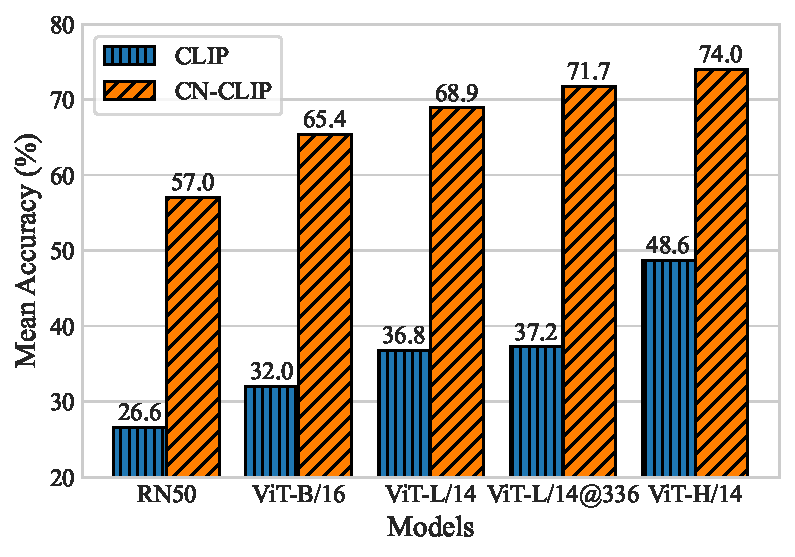
\includegraphics[width=1.0\linewidth]{pics/Mean Recall/cnclip.pdf}
    \caption{\textbf{Comparison of CLIP and Chinese CLIP models on the Chinese native retrieval benchmark MUGE.} On the benchmark based on the native data (which are mostly crawled from the language-native websites, in contrast with the translated data from websites of other countries.), CLIP performs far worse than our Chinese CLIP. Note that $\text{CLIP}\rm_{ViT\text{-}H/14}$ is not released, we use the model from OpenCLIP~\citep{openclip} instead.}
    \label{fig:comparison}
\end{figure}




Starting from the burst of pretraining in NLP, foundation models have attracted attention from multiple research communities. 
Foundation models that learn from large-scale unsupervised or weakly supervised data play as the basis of downstream models. 
% They demonstrate strong transferrability by promoting the downstream performance to a new level~\citep{bert, gpt3}. 
% A series of BERT-based models~\citep{bert, roberta, deberta} have created new state-of-the-art performance in natural language understanding~\citep{glue, superglue}, and the GPT series~\citep{gpt, gpt2, gpt3} and the following language models~\citep{lamda, palm} have demonstrated unprecedented performance in natural language generation, including text generation, dialog, etc. 
% Following natural language pretraining, the transfer of BERT~\citep{bert} and T5~\citep{t5} to multimodal pretraining was also successful~\cite{vilbert, uniter, vinvl, vilt, simvlm, ofa, beit3}. They achieved new state-of-the-art performance in multiple vision-language downstream tasks, e.g., visual question answering, image captioning, cross-modal retrieval, etc. 
% This reflects the great potential of building a foundation model pretrained on large-scale data for cross-modal representation learning. 
A milestone of foundation models~\citep{foundation_model} in multimodal representation learning is CLIP~\cite{clip}. 
Different from the conventional generative pretraining, CLIP is a contrastive-learning-based model pretrained on a large-scale dataset of around $400$ million image-text pair data collected from the web. 
Despite the simplicity of the method, CLIP not only achieved outstanding performance in vision-language retrieval but more importantly played as a vision foundation model and demonstrated state-of-the-art performance in zero-shot image classification across a series of datasets. 
% Furthermore, its simplicity facilitates its application to downstream tasks, and thus we have witnessed a series of studies following or utilizing CLIP, e.g., DALL-E~\cite{dalle, dalle2}, ViLD~\citep{vild}, StyleCLIP~\citep{styleclip}, SLIP~\citep{slip}, CLIP4Clip~\citep{clip4clip}, etc. 
CLIP which builds a connection between vision and language has been transforming the research in both multimodal representation learning and computer vision. 

Be that as it may, it is difficult to efficiently transfer a cross-modal pretrained model to another language for several causes. 
First, learning to model the distribution of language-native vision and language data is significant for the transfer. 
Though CLIP performs as a strong foundation model in most scenarios, we find that it is hard for CLIP with machine translation to perform well on the Chinese-native cross-modal retrieval benchmark.
Figure~\ref{fig:comparison} demonstrates large performance gaps between the original CLIP and our Chinese CLIP at all model scales. 
We assume that it is crucial for both encoders to learn from the language-native images and texts. 
Second, the performance of previous methods for Chinese multimodal pretraining has been inhibited by several factors. Pretraining from scratch requires collecting a large-scale quality language-specific image text pair dataset similar to Web Image Text (WIT) for OpenAI CLIP~\citep{wenlan, r2d2}. Though the fast transfer of CLIP to Chinese data can be realized by using CLIP initialization and Locked-Image Tuning~\citep{lit}, the vision encoder still cannot learn the information of images from the language-specific domains~\citep{wukong}. 
% For example, the Chinese-native data, including both the images and texts crawled from the Chinese websites, reflect information about local features, e.g., cultural values, social customs and landscapes, etc. 

% we find that it is difficult to directly transfer CLIP to language-specific scenarios, say multimodal applications in Chinese, where the data are mostly Chinese-native. 
% A very recent work is mCLIP~\citep{mclip}, which realizes multilingual CLIP by building language-specific text encoders whose output features resemble that of CLIP by training with MSE loss. 
% However, its search engine\footnote{\url{https://rom1504.github.io/clip-retrieval}} fails to return the correct results for the search queries unique to Chinese culture, e.g., ``Spring Festival couplet''. 
% We assume that vision-language foundation models should model the data distribution of the language-specific data so as to transfer to another language. 
% For example, the Chinese-native data, including both the images and texts crawled from the Chinese websites, reflect information about local features, e.g., cultural values, social customs and landscapes, etc. 

Therefore, we propose Chinese CLIP, a language-specific vision-language foundation model pretrained on the publicly available Chinese image-text pair data.  
Additionally, we still use the same architecture as OpenAI CLIP.  
To realize efficient transfer of cross-modal foundation model to Chinese data, we develop a two-stage pretraining method, which is also adaptive to other vision-language foundation models, e.g., ALIGN, Florence, etc. 
Here in this work, we use CLIP as an example. 
To be specific, we first initialize both encoders with pretrained models, namely vision encoders from CLIP and text encoders from RoBERTa-wwm-Chinese~\citep{wwm}. In Stage 1, we freeze the image encoder and only optimize the text encoder with LiT, and in Stage 2, we train both encoders with contrastive tuning~\ref{fig:model}. 
In this way, the new model can inherit from the foundation models through initialization and LiT, and effectively transfer to language-specific data through contrastive tuning. 

% Our ablation study shows that it can achieve improved model performance compared with the other pretraining options. 
We evaluate Chinese CLIP on $3$ Chinese cross-modal retrieval datasets, including MUGE\footnote{\url{https://tianchi.aliyun.com/muge}}, Flickr30K-CN~\citep{flickr30k-cn}, and COCO-CN~\citep{coco-cn}. Experimental results demonstrate that both the large-size and huge-size Chinese CLIP reach state-of-the-art performance on the $3$ datasets in the setups of both zero-shot learning and finetuning. 
Additionally, we evaluate the capability of zero-shot image classification on the track ``Image Classification in the Wild'' of the ELEVATER benchmark~\citep{elevater}. 
% Specifically, we transform the datasets with manual translation for the evaluation of Chinese models.
% \footnote{We will soon release the datasets and templates for prompt ensembling.} 
On the classification datasets, Chinese CLIP demonstrates competitive performance in comparison with state-of-the-art methods and outperforms the Chinese baselines. 
Furthermore, we provide NVIDIA TensorRT and ONNX models for deployments, which run around $2$ to $10$ times faster than Pytorch models for inference. 


% It is pretrained with our proposed two-stage pretraining method on a  large-scale Chinese image-text pair dataset
% We hypothesize that the transfer to language-specific data should significantly boost the performance on the Chinese-native benchmark. 
% Figure~\ref{fig:comparison} shows the performance of CLIP and Chinese CLIP models on MUGE Retrieval, a Chinese-native E-commerce cross-modal retrieval dataset. 
% Note that we apply CLIP by translating texts to English with the in-house automatic translation system. 
% We show that at all model scales, the gaps between CLIP and Chinese CLIP are saliently large. 
% This should be evidence that it is insufficient for the incorporation of a language-agnostic vision-language model and automatic translation to support the cross-modal applications highly relying on language-native data. 
% However, it is still a pity that there is no such model that strictly follows the design of CLIP in the community of Chinese multimodal representation learning. 
% Previous Chinese multimodal pretrained models are mainly generative multiomodal pretrained models~\citep{m6, m6-t, m6-10t}, or contrastive-learning-based models with additional complex model and training task designs~\citep{wenlan, wukong, r2d2}. 
% We assume that it is sufficient for the simple implementation of CLIP on large-scale Chinese data to achieve satisfactory performance in downstream tasks, and we are convinced that the simple architectural design of CLIP is essential to the application of multimodal pretrained models in real-world scenarios. 

% Chinese CLIP models are pretrained on large-scale Chinese image-text pair data. 
% Specifically, we construct a dataset of nearly $200$ million image-text pairs, most of which are publicly available data. 
% To improve the pretraining efficiency and downstream performance, we propose a two-stage method that effectively leverages the existent foundation models. 
% which are retrieved from: the Chinese data in LAION-5B~\citep{schuhmann2021laion}, the Wukong dataset~\citep{wukong}, translated image-text pairs from the publicly available English datasets, and an in-house dataset crawled from the Chinese websites. 
% We build $5$ Chinese CLIP models, ranging from $77$ to $958$ million parameters. 
% which are a tiny-size model with ResNet-50~\citep{resnet} and RBT3~\citep{wwm}, a base-size model with ViT-B/16~\citep{vit} and RoBERTa-wwm-Base~\citep{wwm}, two large-size models with ViT-L/14 and RoBERTa-wwm-Base pretrained on images of $224 \times 224$ and $336 \times 336$ respectively, as well as a huge-size model with ViT-H/14 and RoBERTa-wwm-Large. 
% For the pretraining, we implement a two-stage pretraining method. 

% Also, the tiny-size Chinese CLIP can significantly outperform the large-size baseline. 
% This reflects the potential of the simple architecture and pretraining on large-scale data. 

In brief, our contributions are:
\begin{itemize}
    \item We propose Chinese CLIP, a simple implementation of CLIP pretrained on our collected large-scale Chinese image-text pair data, and we propose a two-stage pretraining method to achieve high pretraining efficiency and improved downstream performance.
    \item Chinese CLIP achieves state-of-the-art performance in cross-modal retrieval in the setups of zero-shot learning and finetuning, and competitive performance in zero-shot image classification. 
    % \item We develop a series of analyses to show the effectiveness of our pretraining method and figure out the inherent problems of Chinese CLIP, e.g., sensitivity to manual prompts, inability to understand negation, etc. 
\end{itemize}
% In the following sections, we introduce the detailed implementation of Chinese CLIP and illustrate the experimental results and analyses of the model. Finally, we review the related work, point out our limitations, and conclude the paper. 
% We believe that the increases in data and model scale can further level up the downstream performance as well as the transferrablity. 


\section{Method}

\begin{figure}[t] 
    \centering
    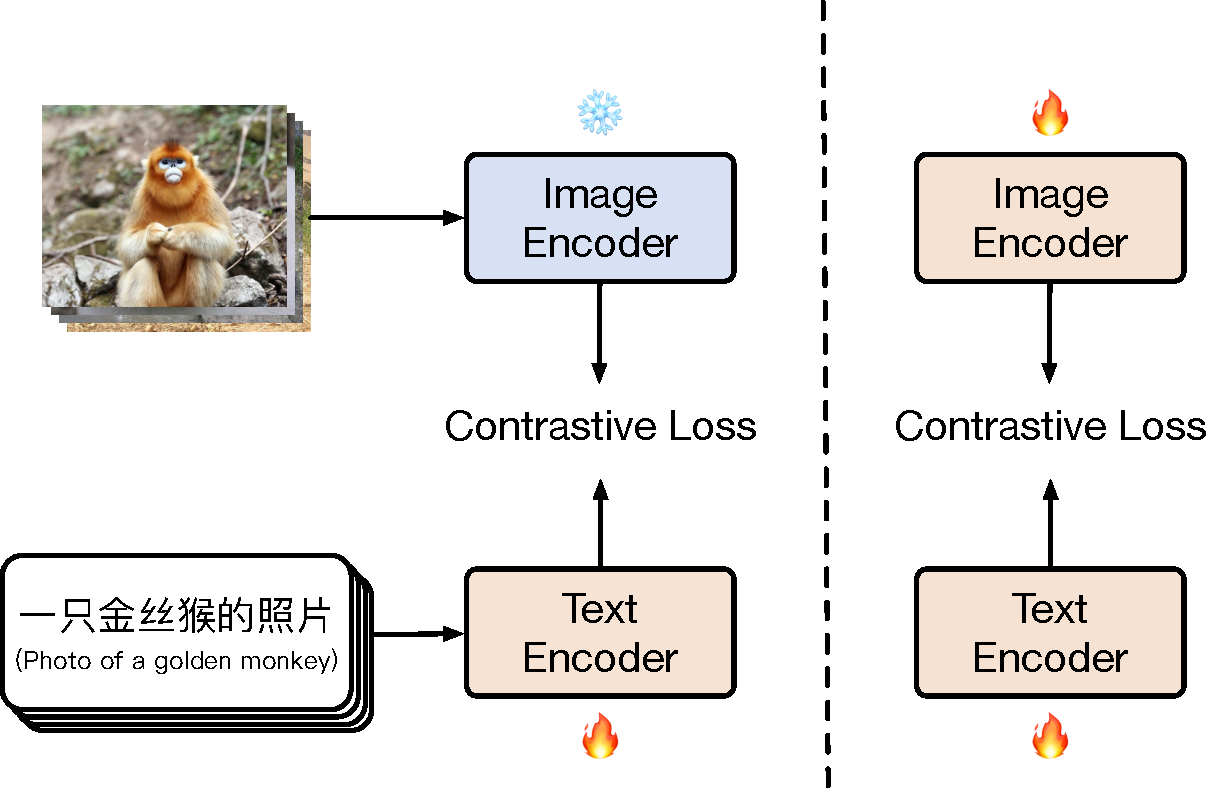
\includegraphics[width=1.0\linewidth]{pics/chinese-clip-model-v3.pdf}
    \caption{\textbf{An illustration of pretraining Chinese CLIP.} To leverage the advantages of the existing pretrained models, we initialize the image encoder with the OpenAI CLIP models, and the text encoder with the Chinese RoBERTa models. In Stage 1, we freeze the weights of the image encoder to avoid weight optimization, and in Stage 2, we unfreeze it and optimize both encoders. }
    \label{fig:model}
\end{figure}

CLIP~\citep{clip} based on simple vision-language contrastive pretraining on large-scale weakly supervised data is a significant foundation model in multimodal representation learning. It can transfer to cross-modal retrieval directly, and its image encoder can play as a vision backbone. 
In this work, we propose to build a language-specific CLIP model by pretraining a vision-language model on large-scale Chinese multimodal data. 
In the following, we provide the details of method design and implementation of our Chinese CLIP. 
% In this section, we first introduce the preliminaries about CLIP and illustrate the details of the data construction and the implementation of Chinese CLIP. 

% \subsection{Preliminaries}

% Before introducing our implementation, we first demonstrate the architecture and training methods of CLIP. 
% CLIP consists of a classical two-tower architecture with an image encoder and a text encoder. 
% An image encoder $\mathcal{M}_{i}$ can be a vision backbone, e.g., ResNet~\cite{resnet}, ViT~\cite{vit}, etc., and a text encoder can be a Transformer model, e.g., BERT~\citep{bert}, GPT~\citep{gpt}, etc. 
% In practice, \citet{clip} proposed CLIP models of multiple model scales with different vision and language backbones. 
% The vision backbones include $5$ ResNets and $3$ ViTs. The $5$ ResNets include ResNet-50, ResNet101, RN50x4, RN50x16, and RN50x64, and the 3 Transformers include ViT-B/32, ViT-B/16, and ViT-L/14. 
% The attention-pooled representation of the top-level features from ResNets or the top-level feature at the $[CLS]$ position from ViTs is treated as the image representation. The top-level feature at the $[EOS]$ position from Transformer is treated as the text representation. 
% To train the model, \citet{clip} applied large-batch contrastive learning. 
% Given $N$ samples in a batch, we have $N \times N$ possible image-text pairs, where there are $N$ positive samples and $N^2 - N$ negative samples. 
% Thus we have $N^2$ similarity scores with inner products of the L2-normalized features and optimize the cross-entropy loss with a learned temperature to control the softmax distribution. 
% CLIP can transfer to cross-modal retrieval directly, and its image encoder can play as a vision backbone. 
%  to replace the original ResNets or ViTs trained on ImageNet~\citep{imagenet}. 
% Furthermore, while CLIP builds a connection between vision and language, it is possible to implement open-vocabulary zero-shot classification by computing similarities between the given image and the candidate labels equipped with a template, e.g., ``a photo of [label]''. To level up the performance in zero-shot image classification, it is a common practice to apply multiple templates to transform a label to multiple sentences, and calculate the mean of the scores of the sentences for a single label. This is also known as prompt ensembling. 

\subsection{Data}
One key to CLIP's success should be the large-scale dataset for pretraining. 
Based on the experiments of a CLIP reimplementation~\citep{openclip}, scaling up data and lengthening the training process can consistently improve the model performance in zero-shot learning. 
This year, the most recent multimodal pretrained models Wukong~\citep{wukong} and R2D2~\citep{r2d2} were pretrained on a public dataset of $100$ million image-text pairs and an in-house dataset of $250$ million samples, where only a subset of $23$ million samples were released. 
For the facility in reimplementation, we aim at pretraining Chinese CLIP on as many publicly available data as possible, and thus we focus on collecting high-quality public datasets. 
We extract the Chinese data (with the mark ``zh'') from the latest LAION-5B~\cite{schuhmann2021laion}, and collect the data from the Wukong dataset. 
However, due to the problems of unavailable links, we can only collect around $108$ million samples and $72$ million samples from LAION-5B and Wukong respectively. 
We additionally add the translated data from the classic English multimodal datasets, including Visual Genome~\cite{vg} and MSCOCO~\citep{coco_cap}, where test sets are removed. 
Finally, we construct a dataset for Chinese multimodal pretraining with around $200$ million image-text pairs.\footnote{We add around $20$ million high-quality internal image-text pairs to provide more diversity. } 
% Furthermore, we add around $20$ million high-quality internal image-text pairs to provide more diversity. 

Below illustrates the procedure for data preprocessing. 
For the part of data from LAION-5B, we remove the samples with CLIP scores lower than $0.26$ computed by mCLIP~\citep{mclip}. 
Besides, we remove the samples with captions containing words in our internal blacklist. 
The blacklist contains words related to advertising, image filenames, etc. 
We remove those samples that are too short (fewer than $5$ characters) or too long (more than $50$ characters). 
For the images, we resize them to the resolution of $224 \times 224$ for most cases and $336 \times 336$ for the ViT-L/14@336px. 

\subsection{Pretraining Method}
\label{subsec:pretraining_method}

There are multiple design choices for pretraining the Chinese CLIP models. 
One of the simplest methods should be pretraining from scratch, where both the image and text encoders are randomly initialized. 
However, we assume that its performance will be limited by the quantity and quality of the current pretraining data. 
To leverage the advantages of existent pretrained models, we initialize the models with weights from the pretrained checkpoints from the official release of CLIP~\footnote{\url{https://github.com/openai/CLIP} License: MIT.} for the image encoder, and RoBERTa-wwm-ext and RBT3~\footnote{\url{https://github.com/ymcui/Chinese-BERT-wwm} License: Apache 2.0} for the text encoder. 
To adapt the model to the introduced pretraining data, it is available to pretrain it with ``contrastive tuning'', similar to the way to transfer CLIP to downstream retrieval data. 
In comparison with contrastive tuning, Locked-image Tuning (LiT)~\citep{lit} demonstrated improved performance in downstream transfer. 

In this work, we propose a two-stage pretraining method, as shown in Figure~\ref{fig:model}. 
The core idea is to first utilize LiT to enable the text encoder to read out high-quality representations from the foundation vision model from OpenAI CLIP, and then transfer the whole model to the domain of the introduced pretraining data. 
It is not sufficient to pretrain Chinese CLIP with solely LiT, as the image encoder should learn the information of the images of the Chinese datasets and model the distribution of such data. 
Before the two-stage pretraining, we first initialize both encoders with pretrained models. 
In Stage 1, we ``lock'' the image encoder by freezing its parameters during pretraining. 
We only pretrain the text encoder for vision-language alignment, based on the assumption that the vision backbone with pretrained weights is already a powerful vision foundation model~\citep{lit, wukong}. 
We pretrain it until there is no salient performance improvement in downstream tasks, even if we prolong the pretraining progress. 
Then we switch to Stage 2, where we ``unlock'' the image encoder by enabling its optimization. 
In Stage 2, we continue pretraining without any parameter frozen, so that the image encoder can learn to model the distribution of the image data from Chinese websites. 
In the ablation study, we discuss the influence of the initialization of the pretrained checkpoints and pretraining methods on the downstream performance. 
Experimental results show that the two-stage pretraining method can outperform either pretraining from scratch or directly finetuning from the pretrained models. 


% \subsection{Scaling}
% \label{subsec:scaling}
% We develop $5$ Chinese CLIP models of different sizes, spanning from around $77$ to $958$ million parameters. 
% We include $1$ ResNet-50 model $\text{CN-CLIP}\rm_{RN50}$ and $4$ ViT models, i.e., $\text{CN-CLIP}\rm_{ViT\text{-}B/16}$, $\text{CN-CLIP}\rm_{ViT\text{-}L/14}$, $\text{CN-CLIP}\rm_{ViT\text{-}L/14@336px}$ and $\text{CN-CLIP}\rm_{ViT\text{-}H/14}$, where models are pretrained on images of the resolution of $224 \times 224$ without specification. 
% Table~\ref{tb:modelcard} presents the details of the model architecture. 
% The smallest model $\text{CN-CLIP}\rm_{RN50}$ consists of a ResNet-50 for the image encoder and a RBT3 for the text encoder. 
% The base-size model $\text{CN-CLIP}\rm_{ViT\text{-}B/16}$ consists of a ViT-B/16@224px for the image encoder and a RoBERTa-wwm-Base for the text encoder. 
% The large-size model $\text{CN-CLIP}\rm_{ViT\text{-}L/14}$ consists of a ViT-L/14@224px for the image encoder and a RoBERTa-wwm-Base for the text encoder, while $\text{CN-CLIP}\rm_{ViT\text{-}L/14@336px}$ consists of a ViT-L/14@336px and a RoBERTa-wwm-Base. 
% Specifically, we pretrain $\text{CN-CLIP}\rm_{ViT\text{-}L/14@336px}$ by continuing pretraining on the pretrained $\text{CN-CLIP}\rm_{ViT\text{-}L/14}$. 
% For the adaptation to a larger resolution, we initialize the image positional embedding by applying interpolation to the positional embedding of $\text{CN-CLIP}\rm_{ViT\text{-}L/14}$, following \citet{openclip}. 
% The huge-size model $\text{CN-CLIP}\rm_{ViT\text{-}H/14}$ consists of a ViT-H/14 for the image encoder and RoBERTa-wwm-Large for the text encoder. 
% More implementation details are presented in Appendix~\ref{sec:implementation_details}.

% \begin{table*}[t]
\center
\small
\vskip 0.15in
\begin{adjustbox}{max width=1.\textwidth}
\begin{tabular}{@{\extracolsep{\fill}}lcccccc}
\toprule
  Model
  & \#Params (All)
  & Backbone (I)
  & \#Params (I)
  & Backbone (T)
  & \#Params (T)
  & Resolution
  \\
\midrule
    $\text{CN-CLIP}\rm_{RN50}$
    & 77M & ResNet-50 & 38M & RBT3 & 39M & $224\times224$
    \\
    $\text{CN-CLIP}\rm_{ViT\text{-}B/16}$
    & 188M & ViT-B/16 & 86M & RoBERTa-wwm-Base & 102M & $224\times224$
    \\
    $\text{CN-CLIP}\rm_{ViT\text{-}L/14}$
    & 406M & ViT-L/14 & 304M & RoBERTa-wwm-Base & 102M & $224\times224$
    \\
    $\text{CN-CLIP}\rm_{ViT\text{-}L/14@336px}$
    & 407M & ViT-L/14 & 304M & RoBERTa-wwm-Base & 102M & $336\times336$
    \\
    $\text{CN-CLIP}\rm_{ViT\text{-}H/14}$
    & 958M & ViT-H/14 & 632M & RoBERTa-wwm-Large & 326M & $224\times224$
    \\
\bottomrule
\end{tabular}
\end{adjustbox}
\caption{Hyperparameters of Chinese CLIP models of different sizes. }
\label{tb:modelcard}
\end{table*}


\begin{table*}[t]
\center
\small
\vskip 0.15in
\begin{adjustbox}{max width=1.\textwidth}
\begin{tabular}{@{\extracolsep{\fill}}lccccccccc}
\toprule
  Tasks
  &\multicolumn{4}{c}{Zero-shot}
  %&COCO Captions
  &\multicolumn{4}{c}{Finetuning}
  \\
\midrule
  Metrics & R@1 & R@5 & R@10 & MR & R@1 & R@5 & R@10 & MR
  \\
\midrule
    \multicolumn{9}{l}{\textit{Tiny}-size Model} \\
    $\text{CN-CLIP}\rm_{RN50}$
    & \textbf{42.6}	& \textbf{68.6}	& \textbf{77.9}	& \textbf{63.0}	& \textbf{48.6}	& \textbf{75.1}	& \textbf{84.0}	& \textbf{69.2}
    \\
\midrule
    \multicolumn{9}{l}{\textit{Base}-size Models} \\
    $\text{Wukong}\rm_{ViT\text{-}B/32}$
    & 33.4	& 59.3	& 69.7	& 54.1	& 39.2	& 66.9	& 77.4	& 61.2
    \\
    $\text{R2D2}\rm_{ViT\text{-}B}$
    & -	& -	& -	& -	& 47.4	& 75.1	& 83.5	& 68.7
    \\
    $\text{CN-CLIP}\rm_{ViT\text{-}B/16}$
    & \textbf{52.1}	& \textbf{76.7}	& \textbf{84.4}	& \textbf{71.1}	& \textbf{58.4}	& \textbf{83.6}	& \textbf{90.0}	& \textbf{77.4}
    \\
\midrule
    \multicolumn{9}{l}{\textit{Large}-size Models} \\
    $\text{Wukong}\rm_{ViT\text{-}L/14}$
    & 42.7	& 69.0	& 78.0	& 63.2	& 52.7	& 77.9	& 85.6	& 72.1
    \\
    $\text{R2D2}\rm_{ViT\text{-}L/14}$
    & 49.5 	& 75.7 	& 83.2	& 69.5	& 60.1 	& 82.9 	& 89.4 	& 77.5
    \\
    $\text{CN-CLIP}\rm_{ViT\text{-}L/14}$
    & 56.3	& 79.8	& 86.2	& 74.1	& 63.3	& 85.6	& 91.3	& 80.1
    \\
    $\text{CN-CLIP}\rm_{ViT\text{-}L/14@336px}$
    & \textbf{59.0}	& \textbf{81.4}	& \textbf{87.8}	& \textbf{76.1}	& \textbf{65.3}	& \textbf{86.7}	& \textbf{92.1}	& \textbf{81.3}
    \\
\midrule
    \multicolumn{9}{l}{\textit{Huge}-size Models} \\
    $\text{CN-CLIP}\rm_{ViT\text{-}H/14}$
    & \textbf{63.0}	& \textbf{84.1}	& \textbf{89.2}	& \textbf{78.8}	& \textbf{68.9}	& \textbf{88.7}	& \textbf{93.1}	& \textbf{83.6}
    \\
\bottomrule
\end{tabular}
\end{adjustbox}
\caption{Experimental results on MUGE-Retrieval. We report the performance of both baselines and Chinese CLIP models on text-to-image retrieval and image-to-text retrieval in the setups of zero-shot evaluation and finetuning. }
\label{tb:muge}
\end{table*}



\begin{table*}[t]
\center
\small
\vskip 0.15in
\begin{adjustbox}{max width=1.\textwidth}
\begin{tabular}{@{\extracolsep{\fill}}lccccccccccccc}
\toprule
  Tasks
  &\multicolumn{6}{c}{Text-to-Image}
  &\multicolumn{6}{c}{Image-to-Text}
  \\
\midrule
  Setups
  &\multicolumn{3}{c}{Zero-shot}
  &\multicolumn{3}{c}{Finetuning}
  &\multicolumn{3}{c}{Zero-shot}
  &\multicolumn{3}{c}{Finetuning}
  \\
\midrule
  Metrics & R@1 & R@5 & R@10 & R@1 & R@5 & R@10 & R@1 & R@5 & R@10 & R@1 & R@5 & R@10
  \\
\midrule
    \multicolumn{13}{l}{\textit{Tiny}-size Model} \\
    $\text{CN-CLIP}\rm_{RN50}$
    & \textbf{48.8}	& \textbf{76.0}	& \textbf{84.6}	& \textbf{66.7} & \textbf{89.4} & \textbf{94.1} & \textbf{60.0}	& \textbf{85.9}	& \textbf{92.0}	& \textbf{84.2}	& \textbf{96.7}	& \textbf{98.0}
    \\
\midrule
    \multicolumn{13}{l}{\textit{Base}-size Models} \\
    $\text{Wukong}\rm_{ViT\text{-}B/32}$
    & 45.7	& 73.8	& 82.2	& 67.6	& 89.6	& 94.2	& 66.2	& 88.7	& 94.3	& 83.9	& 97.6	& 99.0
    \\
    $\text{R2D2}\rm_{ViT\text{-}B}$
    & -	& -	& -	& 78.3	& 94.6	& 97.0	& -	& -	& -	& 92.6	& \textbf{99.1}	& \textbf{99.8}
    \\
    $\text{CN-CLIP}\rm_{ViT\text{-}B/16}$
    & \textbf{62.7}	& \textbf{86.9}	& \textbf{92.8}	& \textbf{79.1}	& \textbf{94.8}	& \textbf{97.4}	& \textbf{74.6}	& \textbf{93.5}	& \textbf{97.1}	& \textbf{93.5}	& 99.0	& 99.5
    \\
\midrule
    \multicolumn{9}{l}{\textit{Large}-size Models} \\
    $\text{Wukong}\rm_{ViT\text{-}L/14}$
    & 51.7	& 78.9	& 86.3	& 77.4 	& 94.5 	& 97.0	& 76.1	& 94.8	& 97.5	& 92.7 	& 99.1 	& 99.6
    \\
    $\text{R2D2}\rm_{ViT\text{-}L/14}$
    & 60.9	& 86.8	& 92.7	& \textbf{84.4} 	& 96.7 	& 98.4	& 77.6	& 96.7	& \textbf{98.9}	& 95.6 	& \textbf{99.8}	& \textbf{100.0}
    \\
    $\text{CN-CLIP}\rm_{ViT\text{-}L/14}$
    & 68.0	& 89.7	& 94.4	& 82.7	& 96.7	& 98.6	& 80.2	& 96.6	& 98.2	& 96.1	& 99.5	& 99.9
    \\
    $\text{CN-CLIP}\rm_{ViT\text{-}L/14@336px}$
    & \textbf{69.0}	& \textbf{90.7}	& \textbf{95.4}	& \textbf{84.4}	& \textbf{97.1}	& \textbf{98.7}	& \textbf{83.3}	& \textbf{97.2}	& 98.5	& \textbf{96.6}	& \textbf{99.8}	& \textbf{100.0}
    \\
\midrule
    \multicolumn{9}{l}{\textit{Huge}-size Models} \\
    $\text{CN-CLIP}\rm_{ViT\text{-}H/14}$
    & \textbf{71.2}	& \textbf{91.4}	& \textbf{95.5}	& \textbf{83.8}	& \textbf{96.9}	& \textbf{98.6}	& \textbf{81.6}	& \textbf{97.5}	& \textbf{98.8}	& \textbf{95.3}	& \textbf{99.7}	& \textbf{100.0}
    \\
\bottomrule
\end{tabular}
\end{adjustbox}
\caption{Experimental results on Flickr30K-CN. We report the performance of both baselines and Chinese CLIP models on text-to-image retrieval and image-to-text retrieval in the setups of zero-shot evaluation and finetuning. }
\label{tb:flickr}
\end{table*}


\begin{table*}[t]
\center
\small
\vskip 0.15in
\begin{adjustbox}{max width=1.\textwidth}
\begin{tabular}{@{\extracolsep{\fill}}lccccccccccccc}
\toprule
  Tasks
  &\multicolumn{6}{c}{Text-to-Image}
  &\multicolumn{6}{c}{Image-to-Text}
  \\
\midrule
  Setups
  &\multicolumn{3}{c}{Zero-shot}
  &\multicolumn{3}{c}{Finetuning}
  &\multicolumn{3}{c}{Zero-shot}
  &\multicolumn{3}{c}{Finetuning}
  \\
\midrule
  Metrics & R@1 & R@5 & R@10 & R@1 & R@5 & R@10 & R@1 & R@5 & R@10 & R@1 & R@5 & R@10 
  \\
\midrule
    \multicolumn{13}{l}{\textit{Tiny}-size Model} \\
    $\text{CN-CLIP}\rm_{RN50}$
    & \color{gray}{48.1}	& \color{gray}{81.3}	& \color{gray}{90.5}	& \textbf{66.8}	& \textbf{91.1}	& \textbf{97.0}	& \color{gray}{51.6}	& \color{gray}{81.2}	& \color{gray}{90.5}	& \textbf{68.4}	& \textbf{93.3}	& \textbf{97.8}
    \\
\midrule
    \multicolumn{13}{l}{\textit{Base}-size Models} \\
    $\text{Wukong}\rm_{ViT\text{-}B/32}$
    & 49.2	& 79.4	& 87.9	& 67.0	& 91.4	& 96.7	& 48.3	& 77.8	& 88.8	& 65.8	& 90.3	& 96.6
    \\
    $\text{R2D2}\rm_{ViT\text{-}B}$
    & -	& -	& -	& 75.1	& 94.2	& 98.1	& -	& -	& -	& 76.1	& 95.3	& 98.5
    \\
    $\text{CN-CLIP}\rm_{ViT\text{-}B/16}$
    & \color{gray}{62.2}	& \color{gray}{86.6}	& \color{gray}{94.9}	& \textbf{77.0}	& \textbf{97.1}	& \textbf{99.0}	& \color{gray}{57.0}	& \color{gray}{84.1}	& \color{gray}{93.6}	& \textbf{77.4}	& \textbf{96.2}	& \textbf{98.9}
    \\
\midrule
    \multicolumn{9}{l}{\textit{Large}-size Models} \\
    $\text{Wukong}\rm_{ViT\text{-}L/14}$
    & 53.4	& 80.2	& 90.1	& 74.0	& 94.4	& 98.1	& 55.2	& 81.0	& 90.6	& 73.3	& 94.0	& 98.0
    \\
    $\text{R2D2}\rm_{ViT\text{-}L/14}$
    & 56.4	& 85.0	& 93.1	& 79.1	& 96.5	& 98.9	& 63.3	& 89.3	& 95.7	& 79.3	& 97.1	& 98.7
    \\
    $\text{CN-CLIP}\rm_{ViT\text{-}L/14}$
     & \color{gray}{64.0}	  & \color{gray}{89.2}	 & \color{gray}{94.4}	 & 78.9	 & 96.3	 & 99.0	 & \color{gray}{60.4}	 & \color{gray}{84.2}	 & \color{gray}{92.9}	 & 80.2	 & 96.7	 & \textbf{99.2}
    \\
    $\text{CN-CLIP}\rm_{ViT\text{-}L/14@336px}$
    & \color{gray}{64.7}	& \color{gray}{89.6}	& \color{gray}{94.6}	& \textbf{80.1}	& \textbf{96.7}	& \textbf{99.2} & \color{gray}{63.4}	& \color{gray}{87.2}	& \color{gray}{94.4}	& \textbf{81.2}	& \textbf{97.2}	& 99.1
    \\
\midrule
    \multicolumn{9}{l}{\textit{Huge}-size Models} \\
    $\text{CN-CLIP}\rm_{ViT\text{-}H/14}$
    & \color{gray}{69.2}	& \color{gray}{89.9}	& \color{gray}{96.1}	& \textbf{81.5}	& \textbf{96.9}	& \textbf{99.1}	& \color{gray}{63.0}	& \color{gray}{86.6}	& \color{gray}{92.9}	& \textbf{83.5}	& \textbf{97.3}	& \textbf{99.2}
    \\    
\bottomrule
\end{tabular}
\end{adjustbox}
\caption{Experimental results on COCO-CN. We report the performance of both baselines and Chinese CLIP models on text-to-image retrieval and image-to-text retrieval in the setups of zero-shot evaluation and finetuning. Since machine translated COCO is included in our pretraining dataset, here the numbers of Chinese CLIP zero-shot performances are shown in gray.}
\label{tb:coco}
\end{table*}

\section{Evaluation}
To comprehensively probe the effects of Chinese CLIP, we follow the conventional practice that we first evaluate its basic capabilities of cross-modal retrieval, i.e. text-to-image retrieval and image-to-text retrieval, in different domains, including e-commerce and the general domain. 
Additionally, as the contrastive-learning-based pretraining builds a foundation vision model that is semantically connected with natural language, we follow \citet{clip} and evaluate its capabilities of zero-shot classification. Specifically, we validate Chinese CLIP on the classification datasets of the ELEVATER benchmark~\citep{elevater}, which is known as ``Image Classification in the Wild (ICinW)''. 

\subsection{Cross-modal Retrieval}
% This section illustrates the datasets and evaluation metrics and reports our experimental results. We also provide an ablation study to show the effectiveness of our proposed two-stage pretraining method. 

\subsubsection{Datasets and Metrics}
We validate Chinese CLIP on $3$ cross-modal retrieval datasets, namely MUGE-Retrieval, Flickr30K-CN~\cite{flickr30k-cn}, and COCO-CN~\cite{coco-cn}. 
MUGE-Retrieval is an image-text retrieval dataset, where data are extracted from Chinese E-commerce websites. 
Flickr30K-CN and COCO-CN are built from the classical datasets Flickr30K and MSCOCO-1K whose texts are translated into Chinese. 
Our evaluation includes setups of zero-shot learning and finetuning. 
For zero-shot learning, we use Chinese CLIP models to compute the similarity scores between images and texts and return the top-$K$ most similar candidates. For finetuning, we finetune the Chinese CLIP models for cross-modal retrieval with contrastive tuning. The evaluation is the same as that in zero-shot learning. 
The evaluation metrics are Recall@$K$, where $K = \{1, 5, 10\}$, and Mean Recall (MR, i.e., the average of Recall@$K$). 
For comparison, we choose the base-size and large-size Wukong and R2D2 as the baselines, which are the previous SOTA models in Chinese multimodal representation learning. 
Following these baselines, we report validation performance on MUGE and test performance on Flickr30K-CN and COCO-CN.
Note that in the setup of finetuning, R2D2\footnote{Since the original paper of R2D2 does not provide the patch size of their base-size model, here we denote the model as $\text{R2D2}\rm_{ViT\text{-}B}$.} is essentially an end-to-end model of retrieval and ranking. 

\subsubsection{Results}
\label{subsubsec:results}
Table~\ref{tb:muge} reports the model performance on MUGE-Retrieval. For the base-size model, $\text{CN-CLIP}\rm_{ViT\text{-}B/16}$ outperforms the baselines on all metrics and in both setups of zero-shot learning and finetuning. 
Specifically, for the base-size models, $\text{CN-CLIP}\rm_{ViT\text{-}B/16}$ surpasses $\text{Wukong}\rm_{ViT\text{-}B/32}$ by $17.0$ MR in zero-shot learning and surpasses $\text{R2D2}\rm_{ViT\text{-}B}$ by $8.7$ MR in finetuning. 
Besides, the tiny model $\text{CN-CLIP}\rm_{RN50}$ can outperform the base-size $\text{Wukong}\rm_{ViT\text{-}B/32}$ by $8.9$ MR in zero-shot learning and $8.0$ MR in finetuning. 

For the large-size models, $\text{CN-CLIP}\rm_{ViT\text{-}L/14}$ can outperform both baselines in all metrics and $\text{CN-CLIP}\rm_{ViT\text{-}L/14@336px}$ pretrained on images of a larger resolution can achieve the state-of-the-art performance. $\text{CN-CLIP}\rm_{ViT\text{-}L/14@336px}$ outperforms $\text{R2D2}\rm_{ViT\text{-}L/14}$ by $6.6$ MR in zero-shot learning and $3.8$ MR in finetuning. 
When scaling to $\text{CN-CLIP}\rm_{ViT\text{-}H/14}$, the performance is further improved. Compared with the best large-size model $\text{CN-CLIP}\rm_{ViT\text{-}L/14@336px}$, $\text{CN-CLIP}\rm_{ViT\text{-}H/14}$ surpasses it by $2.7$ MR in zero-shot learning and $2.3$ MR in finetuning. 

Table~\ref{tb:flickr} and \ref{tb:coco} report the model performance on Flickr30K-CN and COCO-CN. 
We focus on the evaluation of R@1. 
In both datasets, $\text{CN-CLIP}$ achieves better performance than the baselines. 
For the base-size models, in the setup of zero-shot learning of Flickr30K-CN, $\text{CN-CLIP}\rm_{ViT\text{-}B/16}$ surpasses $\text{Wukong}\rm_{ViT\text{-}B/32}$ by $17.0$ R@1 in text-to-image retrieval and $8.4$ R@1 in image-to-text retrieval, and in the finetuning setup, $\text{CN-CLIP}\rm_{ViT\text{-}B/16}$ surpasses $\text{R2D2}\rm_{ViT\text{-}B}$ by $0.8$ R@1 in image retrieval and $0.9$ R@1 in text retrieval. 
Similarly, in the finetuning setup of COCO-CN, $\text{CN-CLIP}\rm_{ViT\text{-}B/16}$ surpasses $\text{R2D2}\rm_{ViT\text{-}B}$ by $1.9$ R@1 in image retrieval and $1.3$ R@1 in text retrieval. For the tiny-size $\text{CN-CLIP}\rm_{RN50}$, it again achieves or surpasses the performance of $\text{Wukong}\rm_{ViT\text{-}B/32}$ in several metrics of Flickr30K-CN and COCO-CN. Specifically, $\text{CN-CLIP}\rm_{RN50}$ surpasses $\text{Wukong}\rm_{ViT\text{-}B/32}$ by $3.1$ R@1 in the zero-shot learning of Flickr30K-CN image retrieval and by $2.6$ R@1 in the finetuning of COCO-CN text retrieval.

For the large-size models, in the zero-shot setup of Flickr30K-CN, $\text{CN-CLIP}\rm_{ViT\text{-}L/14}$ surpasses $\text{Wukong}\rm_{ViT\text{-}L/14}$ by $16.3$ R@1 in text-to-image retrieval and $4.1$ R@1 in image-to-text retrieval. $\text{CN-CLIP}\rm_{ViT\text{-}L/14@336px}$ further improves over $\text{CN-CLIP}\rm_{ViT\text{-}L/14}$ by $1.0$ R@1 in image retrieval and $3.1$ R@1 in text retrieval. In the finetuning setup, $\text{CN-CLIP}\rm_{ViT\text{-}L/14}$ surpasses $\text{R2D2}\rm_{ViT\text{-}L/14}$ by $0.5$ R@1 in text retrieval. $\text{CN-CLIP}\rm_{ViT\text{-}L/14@336px}$ achieves equal performance with $\text{R2D2}\rm_{ViT\text{-}L/14}$ in image retrieval and surpasses it by $1.0$ R@1 in text retrieval. Similarly, in the finetuning setup of COCO-CN, $\text{CN-CLIP}\rm_{ViT\text{-}L/14}$ surpasses $\text{R2D2}\rm_{ViT\text{-}L/14}$ by $0.9$ R@1 in text retrieval. $\text{CN-CLIP}\rm_{ViT\text{-}L/14@336px}$ further surpasses $\text{R2D2}\rm_{ViT\text{-}L/14}$ by $1.0$ in image retrieval and $1.9$ R@1 in text retrieval. 

On Flickr30K-CN and COCO-CN, scaling from $\text{CN-CLIP}\rm_{ViT\text{-}L/14}$ to $\text{CN-CLIP}\rm_{ViT\text{-}H/14}$ improves the performance in almost all the metrics. Specifically, in the zero-shot setup of Flickr30K-CN, $\text{CN-CLIP}\rm_{ViT\text{-}H/14}$ surpasses $\text{CN-CLIP}\rm_{ViT\text{-}L/14}$ by $3.2$ R@1 in image retrieval and $1.4$ R@1 in text retrieval. Moreover, in the finetuning setup of COCO-CN, $\text{CN-CLIP}\rm_{ViT\text{-}H/14}$ even surpasses $\text{CN-CLIP}\rm_{ViT\text{-}L/14@336px}$ with larger image resolution by $1.4$ R@1 in image retrieval and $2.3$ R@1 in text retrieval. 
We also compare our $\text{CN-CLIP}\rm_{ViT\text{-}H/14}$ with a huge CLIP-like model, T-Bletchley\footnote{\url{https://www.microsoft.com/en-us/research/blog/turing-bletchley-a-universal-image-language-representation-model-by-microsoft/}}. This model has $2.5$ billion parameters and is pretrained on billions of multilingual image-caption pairs. In the finetuning setup of COCO-CN, with smaller sizes of model parameters and pretrain dataset, $\text{CN-CLIP}\rm_{ViT\text{-}H/14}$ still surpasses T-Bletchley by $3.9$ MR.

% \begin{figure}
%     \centering
%     \subfigure[]{
%         \label{fig:MUGE IR}
%         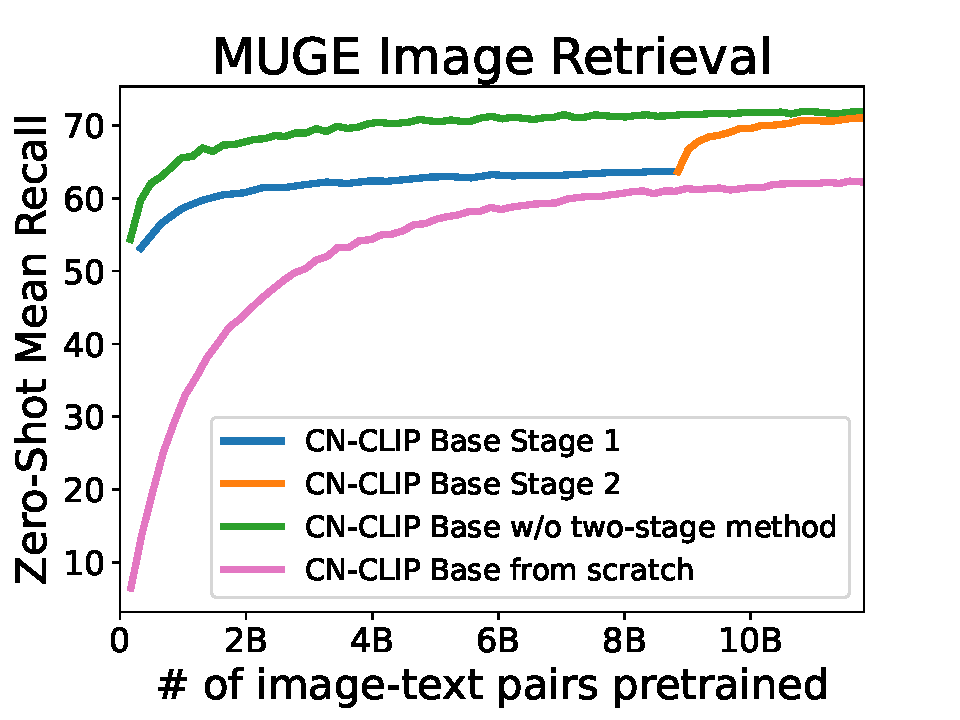
\includegraphics[width=0.97\linewidth]{pics/Mean Recall/MUGE_IR_MR.pdf}
%     }
%     % \caption{Caption}
%     \label{fig:Base MUGE IR}
% \end{figure}
\begin{figure*}
    \centering
    \subfigure[]{
        \begin{minipage}[t]{0.66\columnwidth}
            \label{fig:MUGE IR}
            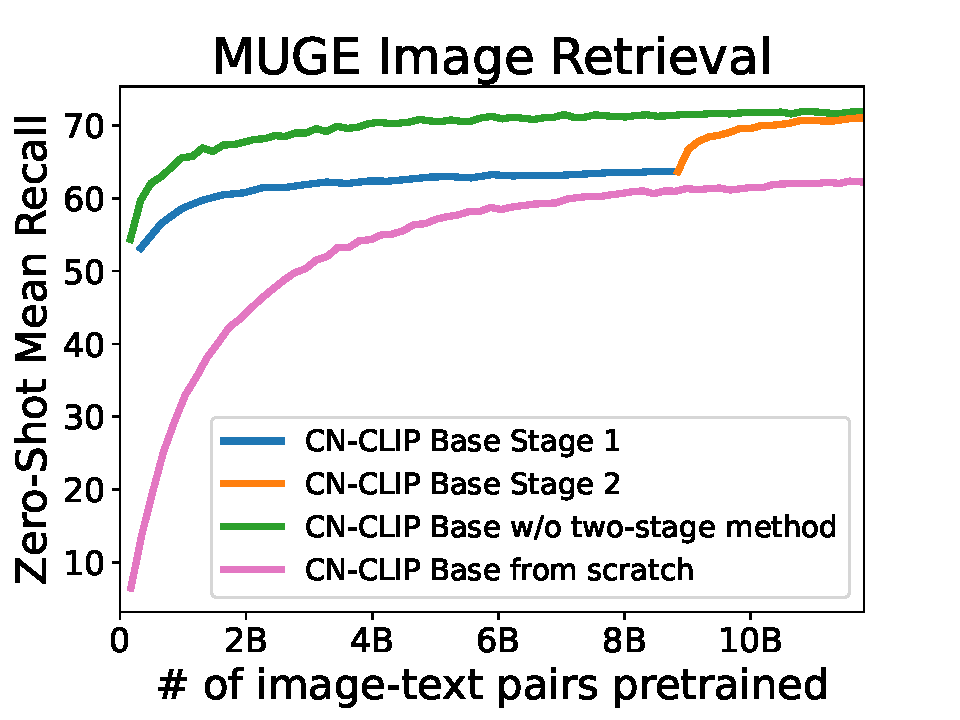
\includegraphics[width=\linewidth]{pics/Mean Recall/MUGE_IR_MR.pdf}
        \end{minipage}
    }
    \subfigure[]{
        \begin{minipage}[t]{0.66\columnwidth}
            \label{fig:Flickr30k-CN IR}
            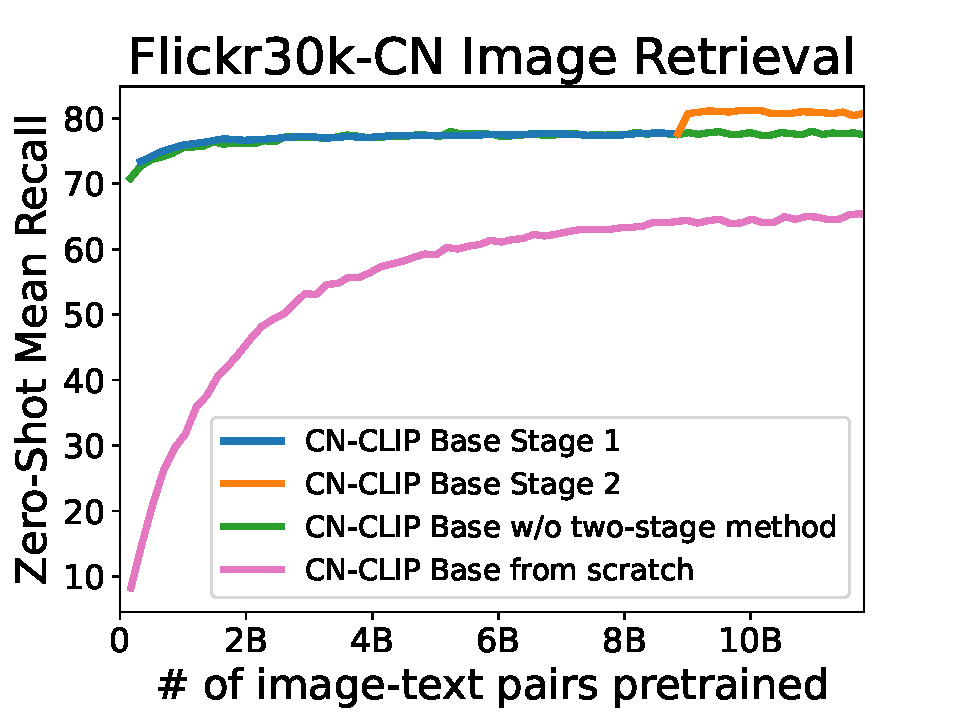
\includegraphics[width=\linewidth]{pics/Mean Recall/Flickr30k-CN_IR_MR.pdf}
        \end{minipage}
    }
    \subfigure[]{
        \begin{minipage}[t]{0.66\columnwidth}
            \label{fig:Flickr30k-CN TR}
            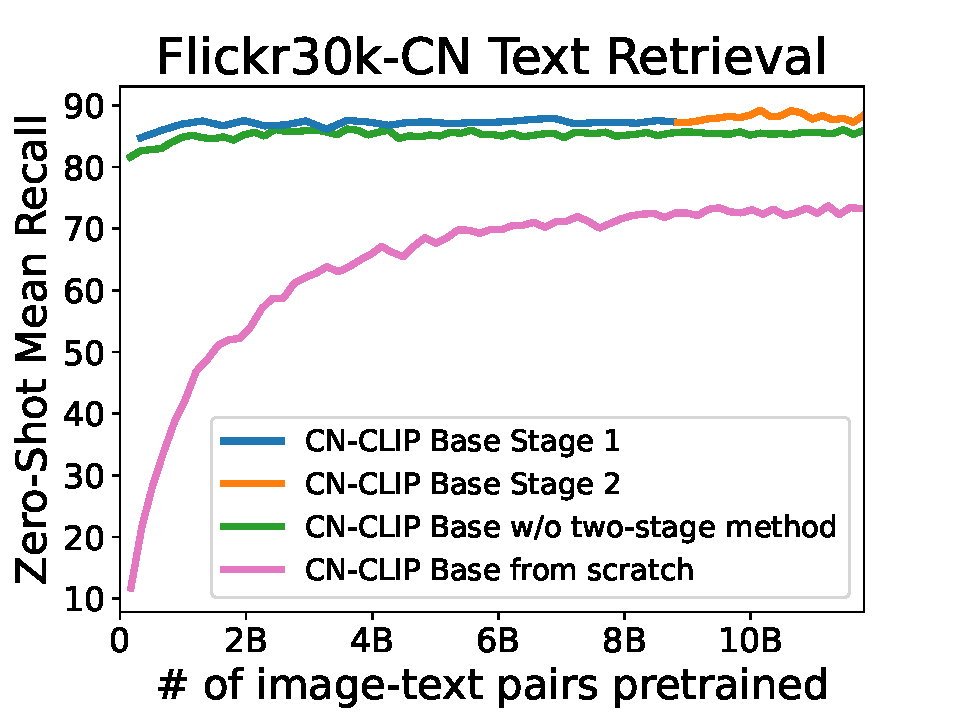
\includegraphics[width=\linewidth]{pics/Mean Recall/Flickr30k-CN_TR_MR.pdf}
        \end{minipage}
    }
    \subfigure[]{
        \begin{minipage}[t]{0.66\columnwidth}
            \label{fig:COCO-CN IR}
            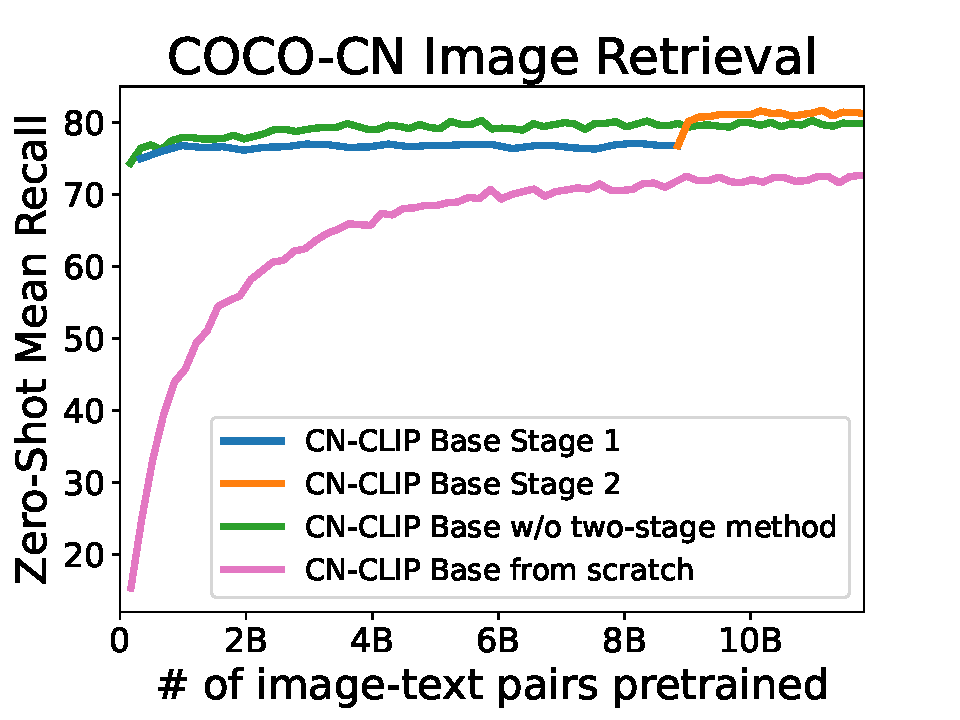
\includegraphics[width=\linewidth]{pics/Mean Recall/COCO-CN_IR_MR.pdf}
        \end{minipage}
    }
    \subfigure[]{
        \begin{minipage}[t]{0.66\columnwidth}
            \label{fig:COCO-CN TR}
            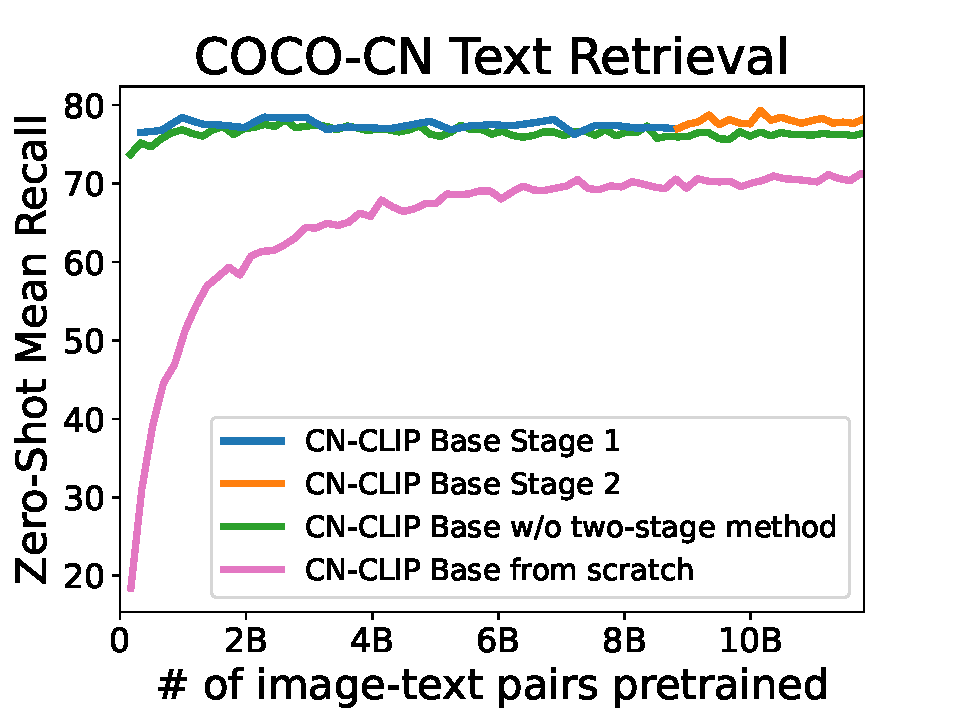
\includegraphics[width=\linewidth]{pics/Mean Recall/COCO-CN_TR_MR.pdf}
        \end{minipage}
    }
    \caption{Comparison of base-size Chinese CLIP models with different training methods on MUGE, Flickr30k-CN and COCO-CN.}
    \label{fig:ablation Base MR}
\end{figure*}

% \begin{figure}
%     \centering
%     \vspace{-0.3cm}
%     \subfigure[]{
%         \begin{minipage}[t]{0.67\linewidth}
%             \label{fig:Flickr30k-CN IR}
%             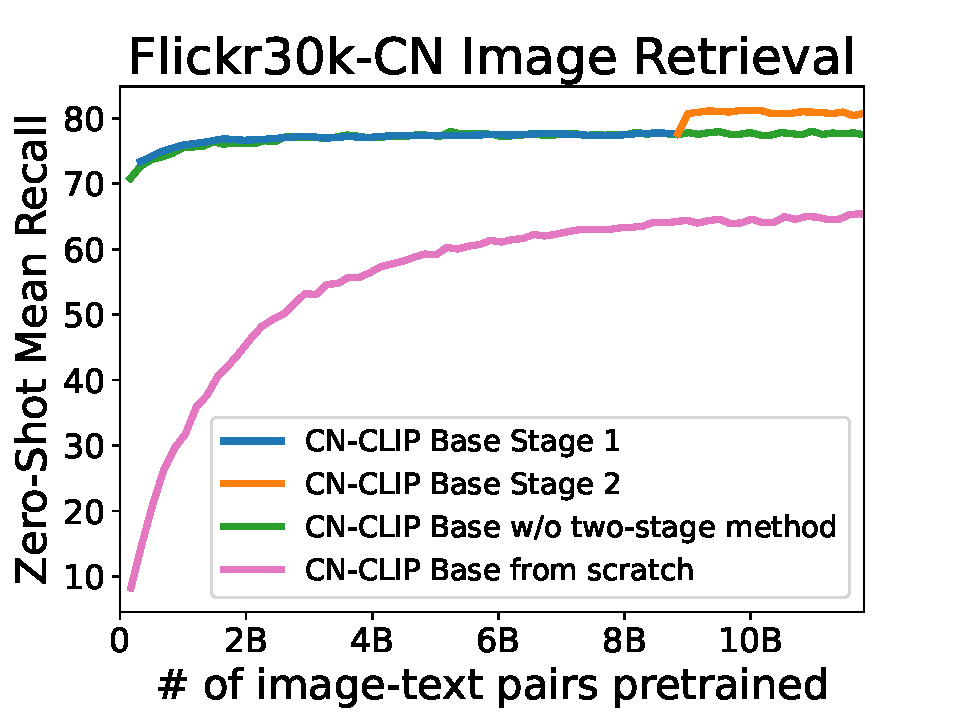
\includegraphics[width=0.97\linewidth]{pics/Mean Recall/Flickr30k-CN_IR_MR.pdf}
%         \end{minipage}
%     }
%     \vspace{-0.3cm}
%     \subfigure[]{
%         \label{fig:Flickr30k-CN TR}
%         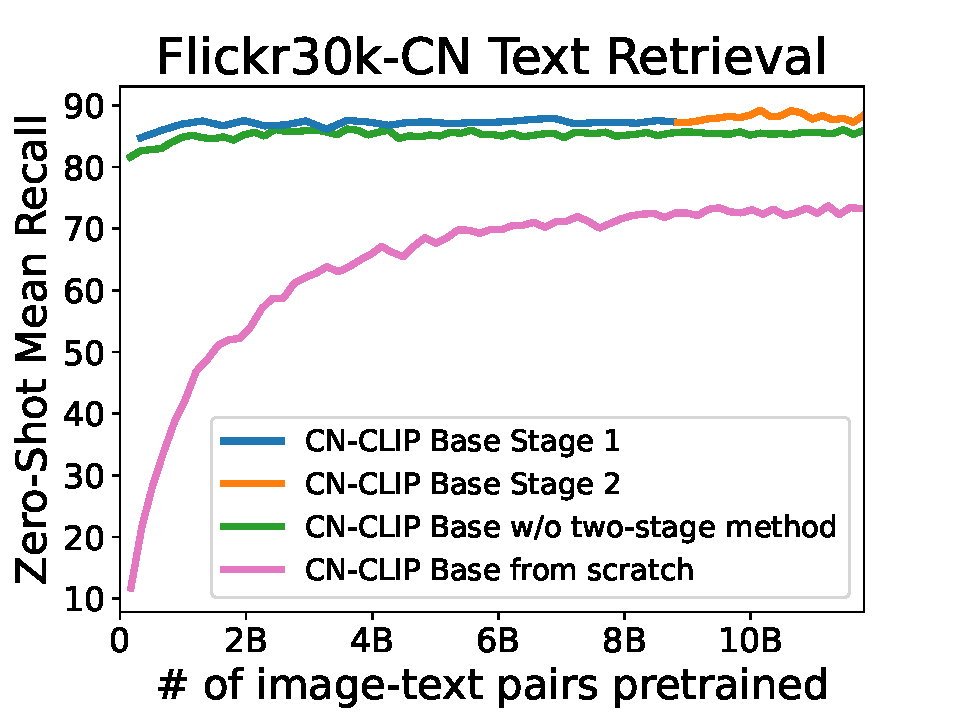
\includegraphics[width=0.97\linewidth]{pics/Mean Recall/Flickr30k-CN_TR_MR.pdf}
%     }
%     \vspace{-0.3cm}
%     \subfigure[]{
%         \label{fig:COCO-CN IR}
%         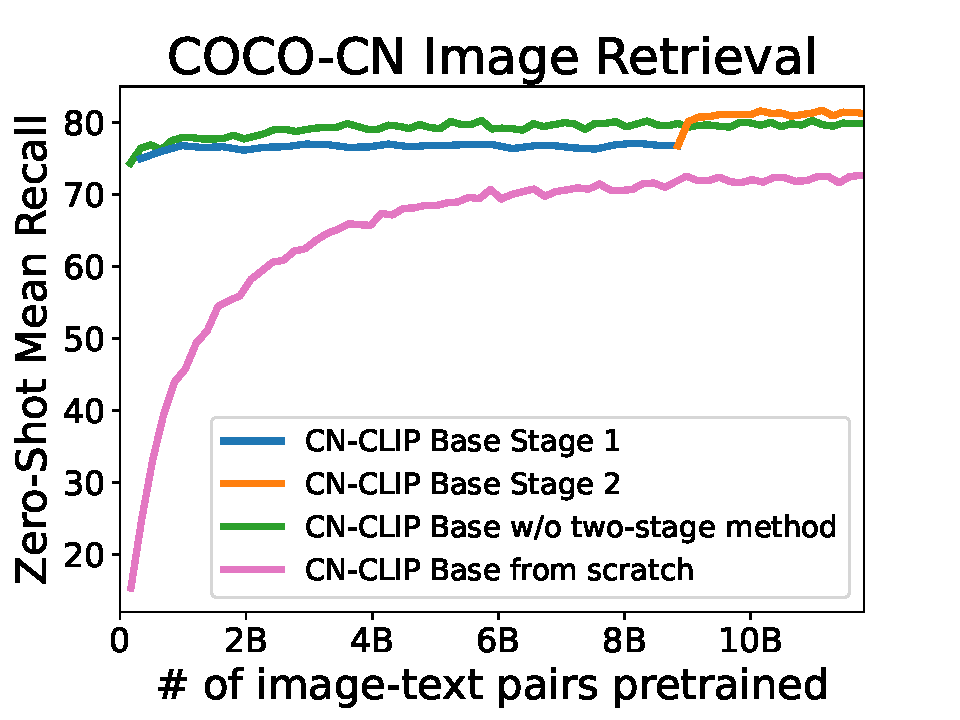
\includegraphics[width=0.97\linewidth]{pics/Mean Recall/COCO-CN_IR_MR.pdf}
%     }
%     \vspace{-0.3cm}
%     \subfigure[]{
%         \label{fig:COCO-CN TR}
%         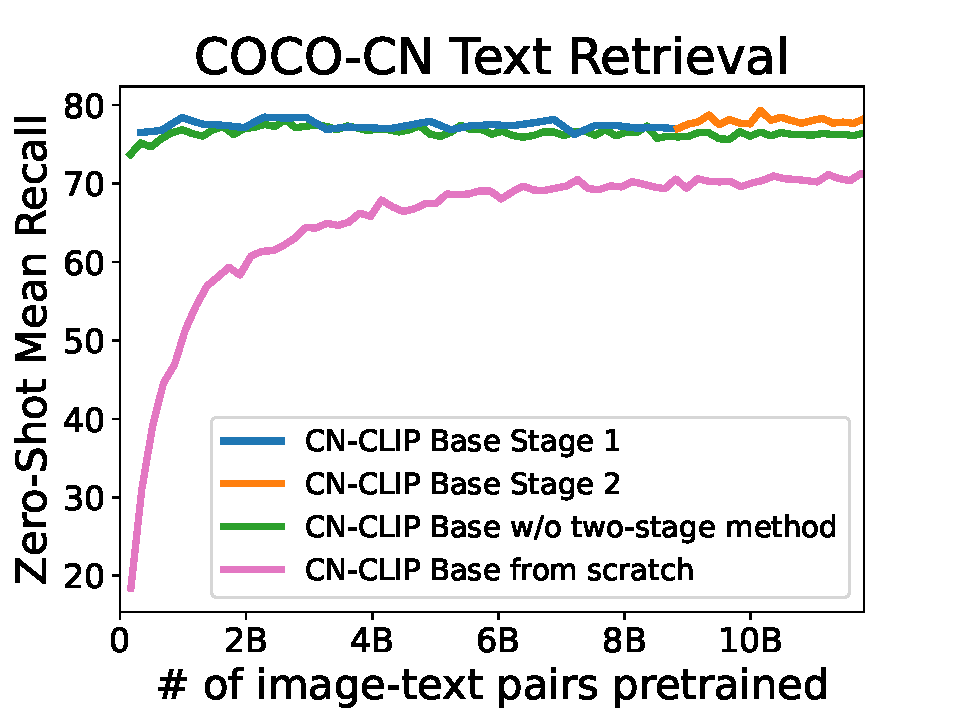
\includegraphics[width=0.97\linewidth]{pics/Mean Recall/COCO-CN_TR_MR.pdf}
%     }
%     \caption{Comparison of the training process of a group of Base scale CLIP models with different training methods on MUGE, Flickr30k-CN and COCO-CN datasets.}
%     \label{fig:Base Flickr30k-CN and COCO-CN MR}
% \end{figure}

\subsubsection{Ablation Study}
Here we provide an ablation study on our proposed two-stage training methods. 
To validate its significance and effectiveness, we design several setups for the ablation study. 
Our experiments are conducted on $\text{CN-CLIP}\rm_{ViT\text{-}B/16}$. 
To evaluate the influence of initialization, we pretrain a model from scratch, and to examine the influence of LiT, we pretrain a model without freezing the image encoder. 
For a better demonstration, we report the curves of model performance of zero-shot retrieval on different datasets in terms of pretraining progress, indicated by the number of processed samples. 

Figure~\ref{fig:ablation Base MR} shows the performance on different tasks, namely MUGE text-to-image retrieval, text-to-image and image-to-text retrieval on Flicrk30K-CN and COCO-CN. 
In comparison with pretraining with pretrained model initialization, pretraining from scratch performs much worse though it shows consistent performance improvement in terms of pretraining progress. 
As to the importance of LiT, we observe different phenomena on different datasets. On MUGE, a dataset of samples originally collected from Chinese websites, we find that pretraining without LiT might be the best solution though its performance gap with two-stage pretraining is quite small. 
However, on the other datasets, i.e., Flickr30K-CN and COCO-CN, whose samples are translated from the English datasets, we find that our two-stage pretraining performs significantly better than pretraining without LiT. 
Furthermore, we observe a common phenomenon that in the two-stage pretraining, switching from Stage 1 to Stage 2 can effectively boost the model performance to a higher level. 
This reflects the importance of adapting the pretrained model to the data distribution of the Chinese multimodal data, especially those concerned with visual information. 

\subsection{Zero-shot Image Classification}
\begin{table*}[t]
\center
\small
\vskip 0.15in
\begin{adjustbox}{max width=1.\textwidth}
\begin{tabular}{@{\extracolsep{\fill}}lccccccccccc}
\toprule
%   Dataset & Metric & $\text{CLIP}\rm_{ViT\text{-}B/32}$ & $\text{CLIP}\rm_{ViT\text{-}B/16}$ & $\text{CLIP}\rm_{ViT\text{-}L/14}$ 
%   & $\text{CN-CLIP}\rm_{RN50}$ & $\text{CN-CLIP}\rm_{ViT\text{-}B/16}$ & $\text{CN-CLIP}\rm_{ViT\text{-}L/14}$ 
%   & $\text{CN-CLIP}\rm_{ViT\text{-}L/14@336px}$ & $\text{CN-CLIP}\rm_{ViT\text{-}H/14}$ 
%   \\
    Model & CIFAR10 & CIFAR100 & DTD & EuroSAT & FER & FGVC & KITTI & MNIST & PC & VOC & INet\\
\midrule
    \multicolumn{8}{l}{\textit{Original benchmark}} \\
    DeCLIP  & 90.9 & 66.8 & 44.9 & 39.9 & 23.3 & 9.0 & 39.7 & 13.6 & 55.3  & 80.6 & 73.7\\
    GIT  & 88.5 & 61.1 & 42.9 & 43.4 & 41.4 & 6.7 & 22.1 & 68.9 & 50.0 & 80.2 & -\\
    % $\text{ALIGN}\rm_{ViT\text{-}B}$ & 88.1 & 60.3 & 44.9 & 14.8 & 46.6 & 62.1 & 53.1 & 82.8\\
    ALIGN & \textbf{94.9} & 76.8 & \textbf{66.1} & 52.1 & \textbf{50.8} & 25.0 & \textbf{41.2} & 74.0 & 55.2 & 83.0 & \textbf{76.4}\\
    % $\text{CLIP}\rm_{ViT\text{-}B/32}$ & Scale & CIFAR-10 & CIFAR-100 & FER & FGVC & KITTI & MNIST & PatchCamelyon & Cars & VOC\\
    OpenCLIP  & 93.5 & 76.2 & 56.4 & 53.7 & 50.3 & 20.8 & 28.8 & 70.9 & 50.5 & 82.3 \\
    CLIP  & \textbf{94.9} & \textbf{77.0} & 56.0 & \textbf{63.0} & 48.3 & \textbf{33.3} & 11.5 &\textbf{79.0} & \textbf{62.3} & \textbf{84.0} & 76.2\\
\midrule
    \multicolumn{8}{l}{\textit{Translated benchmark}} \\
    BriVL  & 72.3 & 35.9 & 18.8 & 25.5 & - & - & - & - & -  & - & 24.3\\
    Wukong & 95.4 & 77.1 & 40.9 & 50.3 & - & - & - & - & -  & - & 55.0\\
    CN-CLIP & \textbf{96.0} & \textbf{79.7} & \textbf{51.2} & \textbf{52.0} & \textbf{55.1} & \textbf{26.2} & \textbf{49.9} & \textbf{79.4} & \textbf{63.5} & \textbf{84.9} & \textbf{59.6} \\
\bottomrule
\end{tabular}
\end{adjustbox}
\caption{Experimental results of the zero-shot image classification performance of models on ICinW. }
\label{tb:zs_v2}
\end{table*}

% Caltech-101 & 87.5 & 88.9 & \textbf{92.4} & 77.3 & 84.9 & 88.5 & 88.8 & 90.6  \\
%   CIFAR-10  & 89.9 & 90.8 & 94.9 & 72.7 & 92.0 & 94.9 & 94.1 & \textbf{96.0}  \\
%   CIFAR-100  & 65.1 & 68.2 & 77.0 & 40.6 & 64.4 & 75.1 & 73.5 & \textbf{79.7}  \\
%   Country-211  & 17.2 & 22.8 & \textbf{34.5} & 7.7 & 15.2 & 21.0 & 25.4 & 25.3  \\
%   DTD  & 44.4 & 44.7 & \textbf{56.0} & 36.9 & 43.6 & 44.2 & 43.8 & 51.2  \\
%   EuroSAT  & 45.6 & 54.7 & \textbf{63.0} & 27.0 & 46.9 & 56.9 & 50.7 & 52.0  \\
%   FER-2013  & 42.1 & 48.5 & 48.3 & 21.9 & 47.2 & 54.6 &\textbf{ 55.1} & 49.2  \\
%   FGVC-Aircraft  & 19.6 & 24.3 & \textbf{33.3} & 5.4 & 12.8 & 16.0 & 17.1 & 26.2  \\
%   Food-101  & 84.0 & 88.7 & \textbf{93.9} & 39.8 & 62.4 & 69.4 & 73.9 & 74.6  \\
%   GTSRB  & 32.8 & 43.6 & \textbf{52.3} & 22.3 & 28.4 & 37.3 & 35.5 & 38.5  \\
%   Hateful-Memes  & 56.0 & 58.1 & \textbf{60.0} & 50.3 & 56.2 & 53.4 & 52.8 & 54.7  \\
%   KITTI-Distance  & 29.0 & 26.7 & 11.5 & 30.2 & 33.5 & 49.9 & \textbf{49.8} & 39.1  \\
%   MNIST  & 48.1 & 52.1 & 79.0 & 50.2 & 67.6 &69.8 & 65.0 & \textbf{79.4}  \\
%   Oxford Flowers-102  & 66.5 & 69.4 & \textbf{78.5} & 30.7 & 52.2 &62.5 & 64.8 & 68.4  \\
%   Oxford-IIIT Pets  & 87.1 & 89.0 & \textbf{93.8} & 48.7 & 73.0 &81.6 & 83.1 & 83.5  \\
%   PatchCamelyon  & 60.7 & 54.0 & 62.3 & 47.7 & 54.0 &\textbf{63.5} & 62.9 & 52.4  \\
%   Rendered-SST2  & 58.4 & 60.6 & \textbf{70.6} & 50.1 & 52.3 & 61.4 & 62.9 & 61.0  \\
%   RESISC-45  & 60.0 & 65.6 & \textbf{71.4} & 49.3 & 58.7 & 65.2 & 65.8 & 66.9  \\
%   Stanford-Cars  & 59.7 & 64.8 & \textbf{79.3} & 27.3 & 42.3 &49.8 & 54.1 & 71.8  \\
%   VOC-2007  & 82.6 & 83.7 & 84.0 & 82.1 & 83.3 & 84.5 & \textbf{84.9} & \textbf{84.9}  \\
%   Average & 56.8 & 60.0 & \textbf{66.8} & 40.9 & 53.5 & 60.0 & 60.2 & 62.3  \\
% This section introduces the image classification datasets, and provides comprehensive experimental results and in-depth analyses to probe the inherent defects of Chinese CLIP. 

\subsubsection{Open-Domain Image Classification Benchmark in Chinese}
Contrastive pretraining on image-text pairs builds a connection between vision and natural language. Natural language supervision instead of crowd-sourced labeling endows models with the capability of zero-shot image classification by computing similarities between the given image and the text descriptions of the labels in the candidate set. 
Recent progress in this field is the ELEVATER benchmark~\citep{elevater}. 
The track ICinW for open-domain image classification consists of a series of image classification datasets, including ImageNet~\citep{imagenet}, CIFAR~\citep{cifar}, MNIST~\citep{mnist}, etc.
%  e.g., CIFAR-10, CIFAR-100~\citep{cifar}, DTD~\citep{dtd}, EuroSAT~\citep{eurosat}, FER-2013~\citep{clip}, FGVC-Aircraft~\citep{fgvc}, KITTI-Distance~\citep{kitti}, MNIST~\citep{mnist}, Pascal-VOC-2007~\citep{voc}, etc. 
% The evaluation metrics include accuracy, mean-per-class, etc. 
% More details about the datasets and metrics are reported in the appendix. 
In order to evaluate Chinese CLIP on the datasets, we first transform the datasets for Chinese models by translating labels and prompts into Chinese. 
% Specifically, we translate the text descriptions of the labels and the templates for manual prompts to Chinese. 
% For example, the labels in CIFAR-10 include ``car, dog, ...'', and we manually translate the words into Chinese. 
% There are also particular cases, such as the labels in FGVC-Aircraft~\citep{fgvc}, which it is difficult to translate or transliterate. 
% We search the names on Google and figure out the best Chinese name for each label. 
% Be that as it may, we cannot guarantee that we have the best Chinese translation, and more importantly, it is still hard for the Chinese pretrained model to understand some of the concepts, which may lead to unsatisfactory performance in the related downstream tasks. 
% As to the templates, for some datasets, we use our translation of the templates provided by the ELEVATER toolkit,\footnote{https://github.com/Computer-Vision-in-the-Wild/Elevater\_Toolkit\_IC} and for the others, we use the translation of the templates from OpenAI CLIP.~\footnote{The organized datasets with translated labels and templates will be released. }

\subsubsection{Experimental Results}
Table~\ref{tb:zs_v2} reports the performance of both English models and Chinese models. 
The baselines pretrained on English data include DeCLIP~\citep{declip}, ALIGN~\citep{align}, CLIP~\citep{clip}, and OpenCLIP~\citep{openclip}, and the baselines pretrained on Chinese data include BriVL~\citep{wenlan} and Wukong~\citep{wukong}. 
We report the results of the variant with the best downstream performance for the models. 

We first focus on the comparison with the Chinese baselines. 
% Chinese CLIP outperforms both baselines on the $4$ datasets significantly. 
% To be specific, Chinese CLIP surpasses BriVL and Wukong by $23.7$ and $0.6$ on CIFAR-10, $43.8$ and $2.6$ on CIFAR-100, $32.4$ and $10.3$ on DTD, and $26.5$ and $1.7$ on EuroSAT. 
To be specific, on all datasets including ImageNet classification, Chinese CLIP surpasses both baselines significantly, and the relative achievements on some datasets are over $100\%$. 
Besides, we also compare Chinese CLIP with the foundation models, e.g., CLIP and ALIGN, which are pretrained on English data. 
It can be found that Chinese CLIP outperforms CLIP or ALIGN on CIFAR-10, CIFAR-100, FER-2013, KITTI-Distance, MNIST, PatchCamelyon, and Pascal-VOC-2007. 
Also, on the classification datasets for general concepts or objects common in both western and eastern culture, Chinese CLIP consistently achieves better performance. 
This indicates that Chinese CLIP is capable of categorizing images to general prototypes. 

However, as to the classification concerned with proper nouns, e.g., FGVC-Aircraft, it is difficult for all models to achieve high accuracy. 
We assume that the related images and texts are not common in the pretraining datasets, and it is also hard for the models to understand the names of airplanes without finetuning. 
Specifically, for Chinese models, the translation or even transliteration can significantly affect the performance of Chinese CLIP. It encourages building a benchmark of ``Image Classification in the Wild for Chinese Models''. 

% Experimental results show that on the $4$ datasets, namely CIFAR-10, CIFAR-100, DTD, and EuroSAT, Chinese CLIP
% The results of the baseline models are provided by the official website of ICinW, which is a direct evaluation of OpenAI CLIP. 
% To be more specific, we report the scores of $\text{CLIP}\rm_{ViT\text{-}B/32}$, $\text{CLIP}\rm_{ViT\text{-}B/16}$, and $\text{CLIP}\rm_{ViT\text{-}L/14@336px}$. 
% As to the average performance on the datasets, the large-size and huge-size Chinese CLIP models, including $\text{CN-CLIP}\rm_{ViT\text{-}L/14}$, $\text{CN-CLIP}\rm_{ViT\text{-}L/14@336px}$, and $\text{CN-CLIP}\rm_{ViT\text{-}H/14}$, can outperform the base-size baselines $\text{CLIP}\rm_{ViT\text{-}B/32}$ and $\text{CLIP}\rm_{ViT\text{-}B/16}$. 
% In comparison with the large-size baseline $\text{CLIP}\rm_{ViT\text{-}L/14@336px}$ pretrained on data of larger resolution $336 \times 336$, the huge-size $\text{CN-CLIP}\rm_{ViT\text{-}H/14}$ outperforms it in several datasets, e.g., CIFAR-10, CIFAR-100, MNIST, and VOC-2007, which are related to the image classification of common objects and general prototypes. 
% This reflects the potential of Chinese CLIP on the understanding of general concepts. 
% Besides, the quality of translation makes a difference in this scenario. 
% There are a number of labels that may not have proper translations in Chinese, or to say, translations that the Chinese language models can understand. 
% For example, most names of airplanes and cars can only be translated into Chinese by transliteration. 
% The language models cannot understand the concepts if their frequencies are low in the corpora. 
% Another problem is that the images of many categories of this benchmark are rare in the Chinese data. 
% To be more specific, many images in some datasets, e.g., Country-211 for country classification, Flowers-102 and Oxford-Pets for the classification of flowers and pets, are quite rare in our pretraining data mostly crawled from the Chinese websites. 
% This finding is consistent with our motivation about why it is necessary to build a language-specific cross-modal pretrained model. 
% Also, it encourages building a benchmark of ``Image Classification in the Wild for Chinese Models''. 


\subsubsection{Analysis}
% Here we illustrate some findings of Chinese CLIP in the experiments, including the sensitivity to handcrafted prompts and the inability to understand negation. 

\paragraph{Sensitivity to Handcrafted Prompts}
While the benchmark ELEVATER provides specific prompts for each dataset, we find that this is not always the best option, in comparison with our baseline, translation of the prompts provided by OpenAI CLIP. 
% Although the accumulation of manual prompts does not consistently improve performance, 
The baseline with around $90$ prompts performs the best on average. 
However, for some datasets, specific prompts designed with human knowledge can boost the performance significantly. 
A typical case is the classification of airplanes. 
We test $\text{CN-CLIP}\rm_{ViT\text{-}L/14}$ with our specified prompts that are related to the knowledge of aircraft, e.g.,``{label}, a photo of an airplane", ``{label}, a zoomed image of a fighter'', etc., and the translation of the OpenAI prompts.
Experimental results show that the model can achieve an accuracy of $16.0$ with the specified prompts but only $13.8$ with the OpenAI prompts. 
% Similar phenomena also happen in other datasets. 
% We list more results in the appendix. 


\paragraph{Inability to Understand Negation}
Previous studies~\citep{negbert, bertnot} demonstrate that even strong NLP pretrained models  often make mistakes in negation problems. 
We explore CLIP's capability to understand negation by conducting experiments on KITTI-Distance~\citep{kitti} and PatchCamelyon~\citep{patchcamelyon}. 
KITTI-Distance provides $4$ options for models to judge, including ``next to a car'', ``near a car'', ``at a distance away from a car'', and ``no car''. The last one is concerned with negation. 
We compare the model performance using the text ``no cars'' and ``others'' for the last label. 
We observe that it is hard for the model to understand negation. By changing the label from ``others'' to ``no cars'', the performance drops by $48.1\%$ in accuracy ($49.9$ vs. $25.9$). 
Similarly, in the experiments on PatchCamelyon, the performance drops from $63.5$ to $50.2$ by changing labels from ``mainly red'' and ``green block in the middle'' to ``no green block in the middle'' and ``green block in the middle''. 
This shows the limitation of the training of CLIP in learning negation. 
The texts in the pretraining datasets are mostly descriptions of the images, which indicate their objects or features but often do not indicate the absence of objects. 
% In the future research, we will explore heuristically building datasets with negation. For example, we sample objects that are not present in an image, construct a text description for negation with manual templates, and train CLIP models on such datasets. 


\subsection{Deployment}
For deployment, we develop ONNX-based and TensorRT-based models based on our Pytorch-based pretrained Chinese CLIP models. 
As expected, we observe that the inference efficiency increases significantly while there is almost no performance sacrifice. 
Specifically, the inference efficiency of TensorRT-based models is around $2$ to $10$ times faster than the Pytorch-based models. More statistics are listed in Appendix~\ref{appendix:deployment}. 

\section{Related Work}
% This section first reviews the related work in general mutlimodal pretraining with a focus on contrastive pretraining, and further reviews the progress of Chinese multimodal pretraining. 

% \paragraph{Multimodal Pretraining}
% There are mainly two lines of studies in multimodal pretraining, namely generative multimodal pretraining and contrastive multimodal pretraining. 
% The core of generative multimodal pretraining is the transfer of BERT or T5 to cross-modal data, and a number of models consecutively created new state-of-the art performance in a series of cross-modal downstream tasks~\citep{uniter, unicoder-vl, visualbert, vilbert, interbert, oscar, pixelbert, e2e-vlp, vinvl, clipvil, simvlm, ofa, albef, blip, mplug, vlmo, beit3}, e.g., image captioning~\citep{coco_cap}, VQA~\citep{vqa, vqav2}, etc. 
Previous vision-language pretrained models are mostly BERT/T5-style~\citep{bert, t5}, which involves cross-modal fusion~\citep{uniter, unicoder-vl, visualbert, vilbert, interbert, oscar, pixelbert, e2e-vlp, vinvl, clipvil, simvlm, ofa, albef, blip, mplug, vlmo, beit3}. 
CLIP~\citep{clip}, instead, is a contrastive-learning-based two-tower model, which can serve as a vision foundation model.  
% CLIP demonstrated that the simple contrastive learning with large-scale multimodal data could build an effective vision foundation model. 
% It revolutionized both computer vision and multimodal representation learning. 
Following CLIP, a series of similar contrastive-learning-based multimodal pretrained models were proposed and reached new SOTAs in cross-modal retrieval and zero-shot classification~\citep{align, filip, florence}. 
Furthermore, CLIP can be adaptive to other models. 
A typical case is that CLIP is essential to many image generation models, e.g., DALL-E~\citep{dalle}, DALL-E 2~\citep{dalle2}, Stable Diffusion~\citep{latent_diffusion}, etc. 
% \paragraph{Chinese Multimodal Pretraining}
The success of multimodal pretraining encouraged the transfer of the existing methods to Chinese pretraining, including generative pretrained models~\citep{m6, wenlan, m6-t, m6-10t, ofa} and contrastive pretrained models~\citep{wenlan, wukong, r2d2, altclip}. 
% Note that in this work, we compare Chinese CLIP with the contrastive-learning-based models, 

% Similarly, researchers have proposed models for both generative and contrastive pretraining. \citet{m6} proposed a model that unifies understanding and generation and pretrained on an in-house large-scale dataset, and further extended it to larger scales~\citep{m6, m6-10t}. 
% \citet{wenlan} started the research in contrastive multimodal pretraining for Chinese data and incorporated complex design for better performance. \citet{wukong} proposed the Wukong dataset, a large-scale public dataset for Chinese multimodal pretraining, and the corresponding pretrained model. 
% \citet{r2d2} proposed a new dataset called ZERO whose subset was released, and pretrained a new model called R2D2 that incorporated contrastive two-tower architecture and interactive module for cross-modal fusion. 
% In this work, different from the previous studies that explored intricate model designs, we build a baseline Chinese CLIP without significant architectural changes from the original CLIP, and we use the simple two-stage pretraining to help Chinese CLIP reach outstanding performance. 




\section{Conclusion}
% This work proposes Chinese CLIP, an implementation of CLIP~\citep{clip} pretrained on large-scale Chinese datasets with contrastive learning. 
In this work, we propose Chinese CLIP, a Chinese-specific vision-language foundation model. 
Specifically, we construct a pretraining dataset of around $200$ million samples, and pretrain a series of Chinese CLIP models with the proposed two-stage pretraining method, which improves both pretraining efficiency and effectiveness. 
% We implement pretraining by initializing encoders with the weights of the existing pretrained models and using our proposed two-stage pretraining method to build $5$ Chinese CLIP models of different model sizes, ranging from $77$ to $958$ million parameters. 
Our comprehensive evaluation shows that Chinese CLIP can reach state-of-the-art performance on multiple cross-modal retrieval datasets in zero-shot learning and finetuning. 
Furthermore, we demonstrate that Chinese CLIP models can also achieve competitive performance in zero-shot image classification across $10$ datasets. 

% In the future, we will explore more efficient methods for pretraining and finetuning Chinese CLIP, and we plan to build vision-language understanding benchmarks based on Chinese-native data, which can better reflect the effectiveness of language-specific vision-language models. 

% However, we still find that Chinese CLIP is limited in some aspects, such as sensitivity to prompts and difficulty in understanding negation. 
% Besides, there is still much room in exploring data scaling and model scaling. 
% In the future, we will continue our research in building Chinese CLIP models with better performance and exploring the features of contrastive-learning-based pretrained models. 

% \section{Introduction}

% These instructions are for authors submitting papers to ACL 2023 using \LaTeX. They are not self-contained. All authors must follow the general instructions for *ACL proceedings,\footnote{\url{http://acl-org.github.io/ACLPUB/formatting.html}} as well as guidelines set forth in the ACL 2023 call for papers.\footnote{\url{https://2023.aclweb.org/calls/main_conference/}} This document contains additional instructions for the \LaTeX{} style files.
% The templates include the \LaTeX{} source of this document (\texttt{acl2023.tex}),
% the \LaTeX{} style file used to format it (\texttt{acl2023.sty}),
% an ACL bibliography style (\texttt{acl\_natbib.bst}),
% an example bibliography (\texttt{custom.bib}),
% and the bibliography for the ACL Anthology (\texttt{anthology.bib}).

% \section{Engines}

% To produce a PDF file, pdf\LaTeX{} is strongly recommended (over original \LaTeX{} plus dvips+ps2pdf or dvipdf). Xe\LaTeX{} also produces PDF files, and is especially suitable for text in non-Latin scripts.
% \begin{table}
% \centering
% \begin{tabular}{lc}
% \hline
% \textbf{Command} & \textbf{Output}\\
% \hline
% \verb|{\"a}| & {\"a} \\
% \verb|{\^e}| & {\^e} \\
% \verb|{\`i}| & {\`i} \\ 
% \verb|{\.I}| & {\.I} \\ 
% \verb|{\o}| & {\o} \\
% \verb|{\'u}| & {\'u}  \\ 
% \verb|{\aa}| & {\aa}  \\\hline
% \end{tabular}
% \begin{tabular}{lc}
% \hline
% \textbf{Command} & \textbf{Output}\\
% \hline
% \verb|{\c c}| & {\c c} \\ 
% \verb|{\u g}| & {\u g} \\ 
% \verb|{\l}| & {\l} \\ 
% \verb|{\~n}| & {\~n} \\ 
% \verb|{\H o}| & {\H o} \\ 
% \verb|{\v r}| & {\v r} \\ 
% \verb|{\ss}| & {\ss} \\
% \hline
% \end{tabular}
% \caption{Example commands for accented characters, to be used in, \emph{e.g.}, Bib\TeX{} entries.}
% \label{tab:accents}
% \end{table}
% \section{Preamble}
% \begin{table*}
% \centering
% \begin{tabular}{lll}
% \hline
% \textbf{Output} & \textbf{natbib command} & \textbf{Old ACL-style command}\\
% \hline
% \citep{ct1965} & \verb|\citep| & \verb|\cite| \\
% \citealp{ct1965} & \verb|\citealp| & no equivalent \\
% \citet{ct1965} & \verb|\citet| & \verb|\newcite| \\
% \citeyearpar{ct1965} & \verb|\citeyearpar| & \verb|\shortcite| \\
% \citeposs{ct1965} & \verb|\citeposs| & no equivalent \\
% \citep[FFT;][]{ct1965} &  \verb|\citep[FFT;][]| & no equivalent\\
% \hline
% \end{tabular}
% \caption{\label{citation-guide}
% Citation commands supported by the style file.
% The style is based on the natbib package and supports all natbib citation commands.
% It also supports commands defined in previous ACL style files for compatibility.
% }
% \end{table*}
% The first line of the file must be
% \begin{quote}
% \begin{verbatim}
% \documentclass[11pt]{article}
% \end{verbatim}
% \end{quote}
% To load the style file in the review version:
% \begin{quote}
% \begin{verbatim}
% \usepackage[review]{ACL2023}
% \end{verbatim}
% \end{quote}
% For the final version, omit the \verb|review| option:
% \begin{quote}
% \begin{verbatim}
% \usepackage{ACL2023}
% \end{verbatim}
% \end{quote}
% To use Times Roman, put the following in the preamble:
% \begin{quote}
% \begin{verbatim}
% \usepackage{times}
% \end{verbatim}
% \end{quote}
% (Alternatives like txfonts or newtx are also acceptable.)
% Please see the \LaTeX{} source of this document for comments on other packages that may be useful.
% Set the title and author using \verb|\title| and \verb|\author|. Within the author list, format multiple authors using \verb|\and| and \verb|\And| and \verb|\AND|; please see the \LaTeX{} source for examples.
% By default, the box containing the title and author names is set to the minimum of 5 cm. If you need more space, include the following in the preamble:
% \begin{quote}
% \begin{verbatim}
% \setlength\titlebox{<dim>}
% \end{verbatim}
% \end{quote}
% where \verb|<dim>| is replaced with a length. Do not set this length smaller than 5 cm.

% \section{Document Body}

% \subsection{Footnotes}

% Footnotes are inserted with the \verb|\footnote| command.\footnote{This is a footnote.}

% \subsection{Tables and figures}

% See Table~\ref{tab:accents} for an example of a table and its caption.
% \textbf{Do not override the default caption sizes.}

% \subsection{Hyperlinks}

% Users of older versions of \LaTeX{} may encounter the following error during compilation: 
% \begin{quote}
% \tt\verb|\pdfendlink| ended up in different nesting level than \verb|\pdfstartlink|.
% \end{quote}
% This happens when pdf\LaTeX{} is used and a citation splits across a page boundary. The best way to fix this is to upgrade \LaTeX{} to 2018-12-01 or later.

% \subsection{Citations}



% Table~\ref{citation-guide} shows the syntax supported by the style files.
% We encourage you to use the natbib styles.
% You can use the command \verb|\citet| (cite in text) to get ``author (year)'' citations, like this citation to a paper by \citet{Gusfield:97}.
% You can use the command \verb|\citep| (cite in parentheses) to get ``(author, year)'' citations \citep{Gusfield:97}.
% You can use the command \verb|\citealp| (alternative cite without parentheses) to get ``author, year'' citations, which is useful for using citations within parentheses (e.g. \citealp{Gusfield:97}).

% \subsection{References}

% \nocite{Ando2005,augenstein-etal-2016-stance,andrew2007scalable,rasooli-tetrault-2015,goodman-etal-2016-noise,harper-2014-learning}

% The \LaTeX{} and Bib\TeX{} style files provided roughly follow the American Psychological Association format.
% If your own bib file is named \texttt{custom.bib}, then placing the following before any appendices in your \LaTeX{} file will generate the references section for you:
% \begin{quote}
% \begin{verbatim}
% \bibliographystyle{acl_natbib}
% \bibliography{custom}
% \end{verbatim}
% \end{quote}
% You can obtain the complete ACL Anthology as a Bib\TeX{} file from \url{https://aclweb.org/anthology/anthology.bib.gz}.
% To include both the Anthology and your own .bib file, use the following instead of the above.
% \begin{quote}
% \begin{verbatim}
% \bibliographystyle{acl_natbib}
% \bibliography{anthology,custom}
% \end{verbatim}
% \end{quote}
% Please see Section~\ref{sec:bibtex} for information on preparing Bib\TeX{} files.

% \subsection{Appendices}

% Use \verb|\appendix| before any appendix section to switch the section numbering over to letters. See Appendix~\ref{sec:appendix} for an example.

% \section{Bib\TeX{} Files}
% \label{sec:bibtex}

% Unicode cannot be used in Bib\TeX{} entries, and some ways of typing special characters can disrupt Bib\TeX's alphabetization. The recommended way of typing special characters is shown in Table~\ref{tab:accents}.

% Please ensure that Bib\TeX{} records contain DOIs or URLs when possible, and for all the ACL materials that you reference.
% Use the \verb|doi| field for DOIs and the \verb|url| field for URLs.
% If a Bib\TeX{} entry has a URL or DOI field, the paper title in the references section will appear as a hyperlink to the paper, using the hyperref \LaTeX{} package.

\section*{Limitations}
A number of issues reflect the limitations of this work but also point out some directions for our future research. In this section, we generally discuss some limitations about the scale of data and model. 

\paragraph{Data} 
The core of CLIP pretraining is the simple but effective large-scale contrastive pretraining on extremely large-scale data. Though we have utilized around $200$ million samples, compared with recent studies~\citep{florence, pali} the scale of our pretraining data is relatively small. 
Thus one of our next-step studies is scaling up the quantity of the pretraining data to evaluate the performance improvement with data scaling. 
Furthermore, we still find it hard to decide what a ``high-quality'' dataset for CLIP is. 
In the previous studies~\citep{align, declip}, the preprocessing methods are mostly simple to avoid the loss of data. 
However, there are still many samples where the image and text are not matched properly, which may provide negative information to the pretraining. 
In our future research, we plan to use the pretrained Chinese CLIP model to compute a score for each image-text pair in a larger dataset, filter those whose scores are under the specified threshold, and pretrain the new models with the new data. 
This is one of the possible solutions to explore the relationship between data quality and pretraining effectiveness. 
Also, such cycling might bring continuous performance enhancement in downstream tasks. 

\paragraph{Model} 
Recently we have witnessed that in many domains the scaling of model size can lead to consistent performance improvement~\citep{scaling_laws,emergent}, and in this work, we also find that the scaling of model size for Chinese CLIP can achieve steady performance improvement in different downstream tasks, including retrieval and classification. 
Recent studies have scaled ViT and also CLIP-like models to a much larger scale than our largest $\text{CN-CLIP}\rm_{ViT\text{-}H/14}$, e.g., the 3B Swin-v2~\citep{swin-v2}, the 4B ViT-e~\citep{pali}, etc. 
In the future, we will continue exploring scaling up models in line with scaling up data in order to build a more effective Chinese CLIP. 

Another issue of model scaling connected with the real-world application is how to build effective small models. 
Experimental results show that our smallest Chinese CLIP $\text{CN-CLIP}\rm_{RN50}$ performs much worse than the ViT variants. 
However, in real-world applications, effective small models that are available for deployment are usually more welcomed. 
Thus it is necessary to explore distillation for CLIP so that the capability of large models can be transferred to small models for application. 


% \section*{Limitations}
% ACL 2023 requires all submissions to have a section titled ``Limitations'', for discussing the limitations of the paper as a complement to the discussion of strengths in the main text. This section should occur after the conclusion, but before the references. It will not count towards the page limit.
% The discussion of limitations is mandatory. Papers without a limitation section will be desk-rejected without review.

% While we are open to different types of limitations, just mentioning that a set of results have been shown for English only probably does not reflect what we expect. 
% Mentioning that the method works mostly for languages with limited morphology, like English, is a much better alternative.
% In addition, limitations such as low scalability to long text, the requirement of large GPU resources, or other things that inspire crucial further investigation are welcome.

\section*{Ethics Statement}
The proposed model is a contrastive-learning-based vision-language foundation model, which generates features for images and texts. Those features can be representation of visual and linguistic information, and they can support applications such as search engine, recommender system, etc. 
Besides, this model can play as a foundation model support recent image generation models, e.g., diffusion models~\citep{dalle2}. 
This may create risks as the AI generated contents may reflect harmful information, such as hate, bias, pornography, etc. 
In most cases, these cases should be attributed to the training of the image generation models. 
Still, we cannot avoid the negative effects from the CLIP representations to the generation. 
In the future, we will study how to filter pretraining data to avoid the potential risks. 

% Our method is essentially based on a generation model, and thus the OCR results should be taken as AI-generated contents. 
% As the generated results should be aligned with the input, we have not noticed deliberate harmful contents, e.g., hate speech, bias, etc.  
% However, the model maintains such ability and it might be triggered. 
% We also have to note that due to the application context, the input may contain harmful contents itself. In such scenario, we believe the model should faithfully reflect its input, which is valuable to measures against such contents.
% Although we believe that after finetuning on the public datasets the risk of such phenomena is extremely low, we still take it into account. 
% In the future research, besides focusing on improving downstream performance, we will study how to increase the controllability on the generation.  

% \section*{Ethics Statement}
% Scientific work published at ACL 2023 must comply with the ACL Ethics Policy.\footnote{\url{https://www.aclweb.org/portal/content/acl-code-ethics}} We encourage all authors to include an explicit ethics statement on the broader impact of the work, or other ethical considerations after the conclusion but before the references. The ethics statement will not count toward the page limit (8 pages for long, 4 pages for short papers).

% \section*{Acknowledgements}
% This document has been adapted by Jordan Boyd-Graber, Naoaki Okazaki, Anna Rogers from the style files used for earlier ACL, EMNLP and NAACL proceedings, including those for
% EACL 2023 by Isabelle Augenstein and Andreas Vlachos,
% EMNLP 2022 by Yue Zhang, Ryan Cotterell and Lea Frermann,
% ACL 2020 by Steven Bethard, Ryan Cotterell and Rui Yan,
% ACL 2019 by Douwe Kiela and Ivan Vuli\'{c},
% NAACL 2019 by Stephanie Lukin and Alla Roskovskaya, 
% ACL 2018 by Shay Cohen, Kevin Gimpel, and Wei Lu, 
% NAACL 2018 by Margaret Mitchell and Stephanie Lukin,
% Bib\TeX{} suggestions for (NA)ACL 2017/2018 from Jason Eisner,
% ACL 2017 by Dan Gildea and Min-Yen Kan, NAACL 2017 by Margaret Mitchell, 
% ACL 2012 by Maggie Li and Michael White, 
% ACL 2010 by Jing-Shin Chang and Philipp Koehn, 
% ACL 2008 by Johanna D. Moore, Simone Teufel, James Allan, and Sadaoki Furui, 
% ACL 2005 by Hwee Tou Ng and Kemal Oflazer, 
% ACL 2002 by Eugene Charniak and Dekang Lin, 
% and earlier ACL and EACL formats written by several people, including
% John Chen, Henry S. Thompson and Donald Walker.
% Additional elements were taken from the formatting instructions of the \emph{International Joint Conference on Artificial Intelligence} and the \emph{Conference on Computer Vision and Pattern Recognition}.

% Entries for the entire Anthology, followed by custom entries
\bibliography{anthology,custom}
\bibliographystyle{acl_natbib}

\newpage
\appendix

\section{Appendix}
\label{sec:implementation_details}

\subsection{Model Architecture Details}
\label{subsec:model_hyperparams}


% \subsection{Scaling}
% \label{subsec:scaling}
We develop $5$ Chinese CLIP models of different sizes, spanning from around $77$ to $958$ million parameters. 
We include $1$ ResNet-50 model $\text{CN-CLIP}\rm_{RN50}$ and $4$ ViT models, i.e., $\text{CN-CLIP}\rm_{ViT\text{-}B/16}$, $\text{CN-CLIP}\rm_{ViT\text{-}L/14}$, $\text{CN-CLIP}\rm_{ViT\text{-}L/14@336px}$ and $\text{CN-CLIP}\rm_{ViT\text{-}H/14}$, where models are pretrained on images of the resolution of $224 \times 224$ without specification. 
Table~\ref{tb:modelcard} presents the details of the model architecture. 
The smallest model $\text{CN-CLIP}\rm_{RN50}$ consists of a ResNet-50 for the image encoder and a RBT3 for the text encoder. 
The base-size model $\text{CN-CLIP}\rm_{ViT\text{-}B/16}$ consists of a ViT-B/16@224px for the image encoder and a RoBERTa-wwm-Base for the text encoder. 
The large-size model $\text{CN-CLIP}\rm_{ViT\text{-}L/14}$ consists of a ViT-L/14@224px for the image encoder and a RoBERTa-wwm-Base for the text encoder, while $\text{CN-CLIP}\rm_{ViT\text{-}L/14@336px}$ consists of a ViT-L/14@336px and a RoBERTa-wwm-Base. 
Specifically, we pretrain $\text{CN-CLIP}\rm_{ViT\text{-}L/14@336px}$ by continuing pretraining on the pretrained $\text{CN-CLIP}\rm_{ViT\text{-}L/14}$. 
For the adaptation to a larger resolution, we initialize the image positional embedding by applying interpolation to the positional embedding of $\text{CN-CLIP}\rm_{ViT\text{-}L/14}$, following \citet{openclip}. 
The huge-size model $\text{CN-CLIP}\rm_{ViT\text{-}H/14}$ consists of a ViT-H/14 for the image encoder and RoBERTa-wwm-Large for the text encoder. 
More implementation details are presented in Appendix~\ref{sec:implementation_details}.

\begin{table*}[t]
\center
\small
\vskip 0.15in
\begin{adjustbox}{max width=1.\textwidth}
\begin{tabular}{@{\extracolsep{\fill}}lcccccc}
\toprule
  Model
  & \#Params (All)
  & Backbone (I)
  & \#Params (I)
  & Backbone (T)
  & \#Params (T)
  & Resolution
  \\
\midrule
    $\text{CN-CLIP}\rm_{RN50}$
    & 77M & ResNet-50 & 38M & RBT3 & 39M & $224\times224$
    \\
    $\text{CN-CLIP}\rm_{ViT\text{-}B/16}$
    & 188M & ViT-B/16 & 86M & RoBERTa-wwm-Base & 102M & $224\times224$
    \\
    $\text{CN-CLIP}\rm_{ViT\text{-}L/14}$
    & 406M & ViT-L/14 & 304M & RoBERTa-wwm-Base & 102M & $224\times224$
    \\
    $\text{CN-CLIP}\rm_{ViT\text{-}L/14@336px}$
    & 407M & ViT-L/14 & 304M & RoBERTa-wwm-Base & 102M & $336\times336$
    \\
    $\text{CN-CLIP}\rm_{ViT\text{-}H/14}$
    & 958M & ViT-H/14 & 632M & RoBERTa-wwm-Large & 326M & $224\times224$
    \\
\bottomrule
\end{tabular}
\end{adjustbox}
\caption{Hyperparameters of Chinese CLIP models of different sizes. }
\label{tb:modelcard}
\end{table*}

\begin{table*}[t]
\center
\small
% \vskip 0.15in
% \begin{adjustbox}{max width=1.\textwidth}
\begin{tabular}{@{\extracolsep{\fill}}lccccccc}
\toprule
  \multirow{2}{*}{Model}
  & Embedding
  & \multicolumn{3}{c}{Vision Transformer}
  & \multicolumn{3}{c}{Text Transformer}
  \\
  & dimension
  & layers
  & width
  & heads
  & layers
  & width
  & heads
  \\
\midrule
    % $\text{CN-CLIP}\rm_{RN50}$
    % & 77M 
    % & ResNet-50 
    % & 38M 
    % & RBT3 
    % & 39M 
    % & $224\times224$
    % \\
    $\text{CN-CLIP}\rm_{ViT\text{-}B/16}$
    & 512
    & 12
    & 768
    & 12
    & 12
    & 768
    & 12
    \\
    $\text{CN-CLIP}\rm_{ViT\text{-}L/14}$
    & 768
    & 24
    & 1,024
    & 16
    & 12
    & 768
    & 12
    \\
    $\text{CN-CLIP}\rm_{ViT\text{-}L/14@336px}$
    & 768
    & 24
    & 1,024
    & 16
    & 12
    & 768
    & 12
    \\
    $\text{CN-CLIP}\rm_{ViT\text{-}H/14}$
    & 1,024
    & 32
    & 1,280
    & 16
    & 24
    & 1,024
    & 24
    \\
\bottomrule
\end{tabular}
% \end{adjustbox}
\caption{Detailed architecture hyperparameters of ViT-based CN-CLIP models.}
\label{tb:detailed_architecture_vit}
\end{table*}

\begin{table*}[t]
\center
\small
% \vskip 0.15in
% \begin{adjustbox}{max width=1.\textwidth}
\begin{tabular}{@{\extracolsep{\fill}}lcccccc}
\toprule
  \multirow{2}{*}{Model}
  & Embedding
  & \multicolumn{2}{c}{ResNet}
  & \multicolumn{3}{c}{Text Transformer}
  \\
  & dimension
  & blocks
  & width
  & layers
  & width
  & heads
  \\
\midrule
    $\text{CN-CLIP}\rm_{RN50}$
    & 1,024
    & (3, 4, 6, 3)
    & 2,048
    & 3
    & 768
    & 12
    \\
\bottomrule
\end{tabular}
% \end{adjustbox}
\caption{Detailed architecture hyperparameters of ResNet-based $\text{CN-CLIP}\rm_{RN50}$.}
\label{tb:detailed_architecture_rn}
\end{table*}
% As mentioned in Section~\ref{subsec:scaling} and Table~\ref{tb:modelcard}, we release $5$ Chinese CLIP models of different sizes. 
We provide more details of their model architectures in Table~\ref{tb:detailed_architecture_vit} and Table~\ref{tb:detailed_architecture_rn}. We keep the architecture of ResNet-50, ViT-B/16, and ViT-L/14 backbones conformed with OpenAI CLIP and the architecture of ViT-H/14 same with LAION CLIP\footnote{\url{https://laion.ai/blog/large-openclip/}}. 
This enables us to initialize the Chinese CLIP image encoders with their weights. 
The text encoders are Chinese Roberta models~\cite{wwm}. Specifically, our most lightweight tiny-size Chinese CLIP uses the architecture of the $3$-layer RBT3 model. The base-size and large-size Chinese CLIP models use the $12$-layer architecture of RoBERTa-wwm-Base. For the huge-size CN-CLIP, we use the $24$-layer architecture of RoBERTa-wwm-Large. The vocabulary size of text tokenizer is $21,128$.

\subsection{Pretraining Details}
\label{subsec:pretraining_details}

\paragraph{Initialization} As mentioned in Section~\ref{subsec:pretraining_method}, we initialize the image encoders of $\text{CN-CLIP}\rm_{RN50}$, $\text{CN-CLIP}\rm_{ViT\text{-}B/16}$ and $\text{CN-CLIP}\rm_{ViT\text{-}L/14}$ using the OpenAI CLIP weights. The image encoder of $\text{CN-CLIP}\rm_{ViT\text{-}H/14}$ is initialized with LAION CLIP. 
Besides the ResNet or ViT parameters, the temperature and visual output projection parameters are also initialized with the pretrained CLIP weights. 
For the text encoder, we initialize the parameters using the released Chinese Roberta weights of the corresponding model scale, with their pooler weights discarded. The text output projection weight is randomly initialized with normal distribution.

\begin{table}[t]
\center
\small
\begin{tabular}{lc}
\toprule
  Hyperparameters
  & Value
  \\
\midrule
    Batch size
    & $32,768$
    \\
    Maximum text length
    & $50$
    \\             
    Peak learning rate
    & $1e-4$
    \\
    Learning rate schedule
    & Cosine
    \\    
    % Training epochs
    % & $20$
    % & $44$
    % & $64$
    % & $26$
    % \\
    Maximum temperature
    & $100$
    \\
    Weight decay
    & $1e-3$
    \\        
    Warmup iterations
    & $5,000$
    \\        
    Adam $\beta_1$
    & $0.9$
    \\      
    Adam $\beta_2$
    & $0.999$ (ResNet), $0.98$ (ViT)
    \\     
    Adam $\epsilon$
    & $1e-8$ (ResNet), $1e-6$ (ViT)
    \\        
\bottomrule
\end{tabular}
\caption{Common pretraining hyperparameters in the first stage.}
\label{tb:hyperparams_stage1}
\end{table}

\paragraph{Stage 1} 
The pretraining hyperparameters of Stage 1 are shown in Table~\ref{tb:hyperparams_stage1}, which are shared for $\text{CN-CLIP}\rm_{RN50}$, $\text{CN-CLIP}\rm_{ViT\text{-}B/16}$, $\text{CN-CLIP}\rm_{ViT\text{-}L/14}$ and $\text{CN-CLIP}\rm_{ViT\text{-}H/14}$. 
The values of hyperparameters are generally similar to those in OpenAI CLIP~\citep{clip}. 
As to data augmentation, we use random resize cropping and AutoAugment~\citep{autoaugment} on input images. We leverage all-gather communications across GPU workers to compute contrastive loss on the global batch. The above $4$ models are pretrained for around $20$, $44$, $64$, and $26$ epochs in this stage respectively, with the image encoder frozen. The running variance and mean of batch normalization layers are not updated in this stage for $\text{CN-CLIP}\rm_{RN50}$. The optimal epochs of pretraining are determined by measuring the mean-recall under the $3$ downstream zero-shot retrieval tasks during training. Mixed-precision training is activated. 
In this stage, we pretrain $1.6$ days using $64$ NVIDIA V100 GPUs for $\text{CN-CLIP}\rm_{RN50}$, $4.5$ days using $128$ NVIDIA V100 GPUs for $\text{CN-CLIP}\rm_{ViT\text{-}B/16}$, $11.5$ days using $128$ NVIDIA V100 GPUs for $\text{CN-CLIP}\rm_{ViT\text{-}L/14}$ and $3.8$ days using $184$ NVIDIA A100 GPUs for $\text{CN-CLIP}\rm_{ViT\text{-}H/14}$.

\paragraph{Stage 2} 
In Stage 2, we unfreeze the image encoder and update all the model parameters. Except for the peak learning rate, batch size and training epochs, all other hyperparameters mentioned in Stage 1 are kept unchanged. We decrease the learning rate to $2e-5$ for subtler optimization. % Updating all the parameters will cost more GPU memory during backward computation. 
For $\text{CN-CLIP}\rm_{RN50}$, $\text{CN-CLIP}\rm_{ViT\text{-}B/16}$ and $\text{CN-CLIP}\rm_{ViT\text{-}L/14}$, the batch size is shrunk to $16,384$, $16,384$ and $4,608$ respectively due to the limitation in GPU memory. When scaling to $\text{CN-CLIP}\rm_{ViT\text{-}H/14}$, we implement gradient checkpointing, which enables a larger batch size of $32,768$. These $4$ models are pretrained for around $44$, $15$, $7$ and $7$ epochs in Stage 2, respectively.
In this stage, we pretrain $\text{CN-CLIP}\rm_{RN50}$ for $5.8$ days using $64$ NVIDIA V100 GPUs, $\text{CN-CLIP}\rm_{ViT\text{-}B/16}$ for $3.0$ days using $128$ NVIDIA V100 GPUs, $\text{CN-CLIP}\rm_{ViT\text{-}L/14}$ for $8.0$ days using $128$ Nvidia V100 GPUs, and $\text{CN-CLIP}\rm_{ViT\text{-}H/14}$ for $2.2$ days using $184$ NVIDIA A100 GPUs. 

To pretrain a model of a larger resolution, we implement interpolation to the image positional embedding of $\text{CN-CLIP}\rm_{ViT\text{-}L/14}$ for adapting to a larger resolution and continue pretraining with images of the resolution of $336 \times 336$. 
We start from $\text{CN-CLIP}\rm_{ViT\text{-}L/14}$ and continue pretraining by $2$ epochs. 
The pretraining only costs the use of $128$ NVIDIA A100 GPUs for $0.7$ days.

\subsection{Finetuning Details}
% % This must be in the first 5 lines to tell arXiv to use pdfLaTeX, which is strongly recommended.
% \pdfoutput=1
% % In particular, the hyperref package requires pdfLaTeX in order to break URLs across lines.

% \documentclass[11pt]{article}

% % Remove the "review" option to generate the final version.
% \usepackage[review]{acl}

% % Standard package includes
% \usepackage{times}
% \usepackage{latexsym}

% % For proper rendering and hyphenation of words containing Latin characters (including in bib files)
% \usepackage[T1]{fontenc}
% % For Vietnamese characters
% % \usepackage[T5]{fontenc}
% % See https://www.latex-project.org/help/documentation/encguide.pdf for other character sets

% % This assumes your files are encoded as UTF8
% \usepackage[utf8]{inputenc}

% This is not strictly necessary, and may be commented out,
% but it will improve the layout of the manuscript,
% and will typically save some space.
% \usepackage{microtype}
% \usepackage{graphicx}
% \usepackage{subfigure}
% \usepackage{booktabs} % for professional tables

% \usepackage{amsfonts}
% \usepackage{stfloats}
% \usepackage{ulem}

% \usepackage{amsmath}
% % Attempt to make hyperref and algorithmic work together better:
% \newcommand{\theHalgorithm}{\arabic{algorithm}}
% \newcommand{\tabincell}[2]{\begin{tabular}{@{}#1@{}}#2\end{tabular}}
% \usepackage{adjustbox}
% \usepackage{multirow}
% \usepackage{array}
% \usepackage{float}
% \usepackage{caption}
% \usepackage{balance}
% \usepackage{flushend}
% \usepackage{color}

% \definecolor{light-gray}{gray}{0.5}
% % If the title and author information does not fit in the area allocated, uncomment the following
% %
% %\setlength\titlebox{<dim>}
% %
% % and set <dim> to something 5cm or larger.

% \title{Chinese CLIP: Contrastive Vision-Language Pretraining in Chinese}
% \begin{document}


\begin{table*}[t]
\center
% \small
% \vskip 0.15in
\begin{adjustbox}{max width=1.\textwidth}
\begin{tabular}{@{\extracolsep{\fill}}lccccccccccccc}
\toprule
  \multirow{2}{*}{Model}
  & \multicolumn{3}{c}{Batch size}
  & \multicolumn{3}{c}{Peak learning rate}
  & \multicolumn{3}{c}{Maximum epochs}
  & \multicolumn{3}{c}{Warmup iterations}

  \\
  & MUGE
  & Flickr
  & COCO
  & MUGE
  & Flickr
  & COCO
  & MUGE
  & Flickr
  & COCO
  & MUGE
  & Flickr
  & COCO
  \\
\midrule
    $\text{CN-CLIP}\rm_{RN50}$
    & 24,576
    & 24,576
    & 24,576
    & 5e-5
    & 6e-5
    & 5e-5
    & 60
    & 30
    & 40
    & 100
    & 20
    & 6
    \\
    $\text{CN-CLIP}\rm_{ViT\text{-}B/16}$
    & 12,800
    & 7,680
    & 12,800
    & 2e-5
    & 5e-5
    & 5e-5
    & 20
    & 16
    & 30
    & 40
    & 20
    & 6
    \\
    $\text{CN-CLIP}\rm_{ViT\text{-}L/14}$
    & 4,096
    & 4,096
    & 4,096
    & 3e-5
    & 2e-5
    & 6e-5
    & 20
    & 16
    & 18
    & 100
    & 60
    & 9
    \\
    $\text{CN-CLIP}\rm_{ViT\text{-}L/14@336px}$
    & 8,192
    & 8,192
    & 8,192
    & 2e-5
    & 2e-5
    & 4e-5
    & 20
    & 18
    & 18
    & 100
    & 20
    & 2
    \\
    $\text{CN-CLIP}\rm_{ViT\text{-}H/14}$
    & 20,480
    & 4,096
    & 5,120
    & 2e-5
    & 6e-6
    & 2e-5
    & 20
    & 18
    & 18
    & 20
    & 6
    & 10
    \\
\bottomrule
\end{tabular}
\end{adjustbox}
\caption{Detailed finetuning hyperparameters of CN-CLIP models.}
\label{tb:detailed_finetune}
\end{table*}

% \end{document}
\begin{table*}[t]
\center
\small
% \vskip 0.15in
\begin{adjustbox}{max width=1.\textwidth}
\begin{tabular}{@{\extracolsep{\fill}}lcccccccc}
\toprule
  Tasks
  &\multicolumn{3}{c}{Text-to-Image}
  &\multicolumn{3}{c}{Image-to-Text}
  & 
  \\
% \midrule
  % Setups
  % &\multicolumn{6}{c}{Finetuning}
  % &\multicolumn{4}{c}{Finetuning}
  % \\
\midrule
  Metrics & R@1 & R@5 & R@10 & R@1 & R@5 & R@10 & MR
  \\
\midrule
  $\text{R2D2}\rm_{ViT\text{-}B}$
  & 42.2    & 69.4  & 77.8	& 43.4	& 69.8	& 78.4 & 63.5
  \\
  $\text{R2D2}\rm_{ViT\text{-}L/14}$
  & 60.7    & 82.0  & 86.9  & 61.5  & 82.9  & 87.7  & 77.0
  \\
  $\text{CN-CLIP}\rm_{ViT\text{-}B/16}$
  & 55.4    & 79.0  & 85.2  & 56.6  & 79.5  & 85.6  & 73.5
  \\
  $\text{CN-CLIP}\rm_{ViT\text{-}L/14}$
  & \textbf{61.6}    & \textbf{83.6}  & \textbf{89.0}  & \textbf{62.5}  & \textbf{83.9}  & \textbf{89.1}  & \textbf{78.3}
  \\

\bottomrule
\end{tabular}
\end{adjustbox}
\caption{Finetuning results on ICR dataset. We report the performance of baselines, $\text{CN-CLIP}\rm_{ViT\text{-}B/16}$ and $\text{CN-CLIP}\rm_{ViT\text{-}L/14}$ on text-to-image and image-to-text retrieval. }
\label{tb:ICR}
\end{table*}
As reported in Table~\ref{tb:muge}, \ref{tb:flickr} and \ref{tb:coco}, we mainly finetune CN-CLIP on $3$ cross-modal retrieval datasets: MUGE, Flickr30K-CN, and COCO-CN.
Most finetuning experiments are conducted on $32$ NVIDIA A100 GPUs.
The finetuning strategy and loss are consistent with the pretraining process.
For time efficiency and full utilization of computation resources, we set the batch size as large as possible.
We implement gradient checkpointing in the finetuning process of $\text{CN-CLIP}\rm_{ViT\text{-}L/14@336px}$ and $\text{CN-CLIP}\rm_{ViT\text{-}H/14}$ for a larger batch size.
Table~\ref{tb:detailed_finetune} shows the specific settings of batch size, peaking learning rate, maximum epochs, and warmup iterations in the finetuning process.
We set other hyperparameters to be the same as those in pretraining by default.
We save the model parameters at the end of each epoch.
For MUGE, we report the best results on the validation set.
For Flickr30K-CN and COCO-CN, we choose the checkpoint with the best performance on the validation set and report the results on the test set.
% In particular, we find that under the same setting of batch size, a larger peak learning rate will lead to , but usually will also reach a higher MR. A relatively small peak learning rate will delay the occurrence of over fitting, but the maximum MR can be lower.


\subsection{Cross-modal Retrieval with Longer Texts}
The results reported in Section~\ref{subsubsec:results} demonstrate the excellent cross-modal retrieval capability of Chinese CLIP.
Note that the average text lengths of MUGE, Flickr30K-CN, and COCO-CN are $7.4$, $19.7$, and $16.8$, respectively.
We also conduct finetuning experiments on the ICR~\citep{r2d2} dataset with an average text length of $45.3$. 
Experimental results are shown in Table~\ref{tb:ICR}.
Since the texts in the ICR dataset are longer, we set the maximum text length to $128$ for finetuning.
The results show that Chinese CLIP achieves state-of-the-art performance in cross-modal retrieval tasks with longer texts.

% We also conducted finetuning experiments on ICR~\citep{r2d2} dataset for $\text{CN-CLIP}\rm_{ViT\text{-}B/16}$ and $\text{CN-CLIP}\rm_{ViT\text{-}L/14}$. Since the text in the ICR dataset is longer, we set the maximum text length to $128$ when finetuning. $\text{CN-CLIP}\rm_{ViT\text{-}B/16}$ and $\text{CN-CLIP}\rm_{ViT\text{-}L/14}$ achieve $73.5$ and $78.3$ 


\subsection{Details About Experiments on Zero-shot Image Classification}

\begin{table*}[t]
\center
\small
\vskip 0.15in
\begin{adjustbox}{max width=1.\textwidth}
\begin{tabular}{@{\extracolsep{\fill}}lccc}
\toprule
%   Dataset & Metric & $\text{CLIP}\rm_{ViT\text{-}B/32}$ & $\text{CLIP}\rm_{ViT\text{-}B/16}$ & $\text{CLIP}\rm_{ViT\text{-}L/14}$ 
%   & $\text{CN-CLIP}\rm_{RN50}$ & $\text{CN-CLIP}\rm_{ViT\text{-}B/16}$ & $\text{CN-CLIP}\rm_{ViT\text{-}L/14}$ 
%   & $\text{CN-CLIP}\rm_{ViT\text{-}L/14@336px}$ & $\text{CN-CLIP}\rm_{ViT\text{-}H/14}$ 
%   \\
Dataset & \#Labels & Test Size & Metric \\
\midrule
  Caltech-101~\citep{caltech} & 101 & 6,084 & Mean-per-class  \\
  CIFAR-10~\citep{cifar} & 10 & 10,000 &  Accuracy   \\
  CIFAR-100~\citep{cifar} & 100 & 10,000 & Accuracy   \\
  Country-211~\citep{clip} & 211 & 21,100 & Accuracy   \\
  DTD~\citep{dtd} & 47 & 1,880 & Accuracy  \\
  EuroSAT~\citep{eurosat} & 10 & 5,000 & Accuracy  \\
  FER-2013~\citep{clip} & 7 & 3,589 & Accuracy  \\
  FGVC-Aircraft~\citep{fgvc} & 100 & 3,333 & Mean-per-class \\
  Food-101~\citep{food101} & 101 & 25,250 & Accuracy \\
  GTSRB~\citep{gtsrb} & 43 & 12,630 & Accuracy  \\
  Hateful-Memes~\citep{hateful} & 2  & 500 & ROC AUC \\
  KITTI-Distance~\citep{kitti} & 4 & 711 & Accuracy  \\
  MNIST~\citep{mnist} & 10 & 10,000 & Accuracy \\
  Oxford Flowers-102~\citep{flowers} & 102 & 6,149 & Mean-per-class  \\
  Oxford-IIIT Pets~\cite{pets} & 37 & 3,669 & Mean-per-class \\
  PatchCamelyon~\citep{patchcamelyon} & 2 & 32,768 & Accuracy  \\
  Rendered-SST2~\citep{clip} & 2 & 1,821 & Accuracy  \\
  RESISC-45~\citep{resisc45} & 45 & 25,200 & Accuracy \\
  Stanford-Cars~\citep{stanford_cars} & 196 & 8,041 & Accuracy  \\
  Pascal VOC-2007~\citep{voc} & 20 & 4,952 & 11-point mAP \\
\bottomrule
\end{tabular}
\end{adjustbox}
\caption{Details of the image classification datasets in the ELEVATER benchmark. }
\label{tb:icinw}
\end{table*}

\begin{table*}[t]
\center
\small
\vskip 0.15in
\begin{adjustbox}{max width=1.\textwidth}
\begin{tabular}{@{\extracolsep{\fill}}lccccc}
\toprule
%   Dataset & Metric & $\text{CLIP}\rm_{ViT\text{-}B/32}$ & $\text{CLIP}\rm_{ViT\text{-}B/16}$ & $\text{CLIP}\rm_{ViT\text{-}L/14}$ 
%   & $\text{CN-CLIP}\rm_{RN50}$ & $\text{CN-CLIP}\rm_{ViT\text{-}B/16}$ & $\text{CN-CLIP}\rm_{ViT\text{-}L/14}$ 
%   & $\text{CN-CLIP}\rm_{ViT\text{-}L/14@336px}$ & $\text{CN-CLIP}\rm_{ViT\text{-}H/14}$ 
%   \\
\multirow{2}{*}{Dataset} & CN-CLIP & CN-CLIP & CN-CLIP & CN-CLIP & CN-CLIP \\
 & $\rm_{RN50}$ & $\rm_{ViT\text{-}B/16}$ & $\rm_{ViT\text{-}L/14}$ & $\rm_{ViT\text{-}L/14@336px}$ & $\rm_{ViT\text{-}H/14}$ \\
\midrule
  Caltech-101  & 77.3 & 84.9 & 88.5 & 88.8 & 90.6  \\
  CIFAR-10  & 72.7 & 92.0 & 94.9 & 94.1 & 96.0  \\
  CIFAR-100   & 40.6 & 64.4 & 75.1 & 73.5 & 79.7  \\
  Country-211   & 7.7 & 15.2 & 21.0 & 25.4 & 25.3  \\
  DTD   & 36.9 & 43.6 & 44.2 & 43.8 & 51.2  \\
  EuroSAT   & 27.0 & 46.9 & 56.9 & 50.7 & 52.0  \\
  FER-2013   & 21.9 & 47.2 & 54.6 & 55.1 & 49.2  \\
  FGVC-Aircraft  & 5.4 & 12.8 & 16.0 & 17.1 & 26.2  \\
  Food-101   & 39.8 & 62.4 & 69.4 & 73.9 & 74.6  \\
  GTSRB   & 22.3 & 28.4 & 37.3 & 35.5 & 38.5  \\
  Hateful-Memes   & 50.3 & 56.2 & 53.4 & 52.8 & 54.7  \\
  KITTI-Distance  & 30.2 & 33.5 & 49.9 & 49.8 & 39.1  \\
  MNIST   & 50.2 & 67.6 &69.8 & 65.0 & 79.4  \\
  Oxford Flowers-102   & 30.7 & 52.2 &62.5 & 64.8 & 68.4  \\
  Oxford-IIIT Pets   & 48.7 & 73.0 &81.6 & 83.1 & 83.5  \\
  PatchCamelyon  & 47.7 & 54.0 & 63.5 & 62.9 & 52.4  \\
  Rendered-SST2  & 50.1 & 52.3 & 61.4 & 62.9 & 61.0  \\
  RESISC-45   & 49.3 & 58.7 & 65.2 & 65.8 & 66.9  \\
  Stanford-Cars  & 27.3 & 42.3 &49.8 & 54.1 & 71.8  \\
  VOC-2007  & 82.1 & 83.3 & 84.5 & 84.9 & 84.9  \\
  Average  & 40.9 & 53.5 & 60.0 & 60.2 & 62.3  \\
\bottomrule
\end{tabular}
\end{adjustbox}
\caption{Experimental results of the zero-shot image classification performance of models on ICinW. }
\label{tb:zs}
\end{table*}

% \begin{table*}[t]
% \center
% \small
% \vskip 0.15in
% \begin{adjustbox}{max width=1.\textwidth}
% \begin{tabular}{@{\extracolsep{\fill}}lcccccccc}
% \toprule
% %   Dataset & Metric & $\text{CLIP}\rm_{ViT\text{-}B/32}$ & $\text{CLIP}\rm_{ViT\text{-}B/16}$ & $\text{CLIP}\rm_{ViT\text{-}L/14}$ 
% %   & $\text{CN-CLIP}\rm_{RN50}$ & $\text{CN-CLIP}\rm_{ViT\text{-}B/16}$ & $\text{CN-CLIP}\rm_{ViT\text{-}L/14}$ 
% %   & $\text{CN-CLIP}\rm_{ViT\text{-}L/14@336px}$ & $\text{CN-CLIP}\rm_{ViT\text{-}H/14}$ 
% %   \\
% \multirow{2}{*}{Dataset} & CLIP & CLIP & CLIP & CN-CLIP & CN-CLIP & CN-CLIP & CN-CLIP & CN-CLIP \\
%  & $\rm_{ViT\text{-}B/32}$ & $\rm_{ViT\text{-}B/16}$ & $\rm_{ViT\text{-}L/14@336px}$ & $\rm_{RN50}$ & $\rm_{ViT\text{-}B/16}$ & $\rm_{ViT\text{-}L/14}$ & $\rm_{ViT\text{-}L/14@336px}$ & $\rm_{ViT\text{-}H/14}$ \\
% \midrule
%   Caltech-101 & 87.5 & 88.9 & \textbf{92.4} & 77.3 & 84.9 & 88.5 & 88.8 & 90.6  \\
%   CIFAR-10  & 89.9 & 90.8 & 94.9 & 72.7 & 92.0 & 94.9 & 94.1 & \textbf{96.0}  \\
%   CIFAR-100  & 65.1 & 68.2 & 77.0 & 40.6 & 64.4 & 75.1 & 73.5 & \textbf{79.7}  \\
%   Country-211  & 17.2 & 22.8 & \textbf{34.5} & 7.7 & 15.2 & 21.0 & 25.4 & 25.3  \\
%   DTD  & 44.4 & 44.7 & \textbf{56.0} & 36.9 & 43.6 & 44.2 & 43.8 & 51.2  \\
%   EuroSAT  & 45.6 & 54.7 & \textbf{63.0} & 27.0 & 46.9 & 56.9 & 50.7 & 52.0  \\
%   FER-2013  & 42.1 & 48.5 & 48.3 & 21.9 & 47.2 & 54.6 &\textbf{ 55.1} & 49.2  \\
%   FGVC-Aircraft  & 19.6 & 24.3 & \textbf{33.3} & 5.4 & 12.8 & 16.0 & 17.1 & 26.2  \\
%   Food-101  & 84.0 & 88.7 & \textbf{93.9} & 39.8 & 62.4 & 69.4 & 73.9 & 74.6  \\
%   GTSRB  & 32.8 & 43.6 & \textbf{52.3} & 22.3 & 28.4 & 37.3 & 35.5 & 38.5  \\
%   Hateful-Memes  & 56.0 & 58.1 & \textbf{60.0} & 50.3 & 56.2 & 53.4 & 52.8 & 54.7  \\
%   KITTI-Distance  & 29.0 & 26.7 & 11.5 & 30.2 & 33.5 & 49.9 & \textbf{49.8} & 39.1  \\
%   MNIST  & 48.1 & 52.1 & 79.0 & 50.2 & 67.6 &69.8 & 65.0 & \textbf{79.4}  \\
%   Oxford Flowers-102  & 66.5 & 69.4 & \textbf{78.5} & 30.7 & 52.2 &62.5 & 64.8 & 68.4  \\
%   Oxford-IIIT Pets  & 87.1 & 89.0 & \textbf{93.8} & 48.7 & 73.0 &81.6 & 83.1 & 83.5  \\
%   PatchCamelyon  & 60.7 & 54.0 & 62.3 & 47.7 & 54.0 &\textbf{63.5} & 62.9 & 52.4  \\
%   Rendered-SST2  & 58.4 & 60.6 & \textbf{70.6} & 50.1 & 52.3 & 61.4 & 62.9 & 61.0  \\
%   RESISC-45  & 60.0 & 65.6 & \textbf{71.4} & 49.3 & 58.7 & 65.2 & 65.8 & 66.9  \\
%   Stanford-Cars  & 59.7 & 64.8 & \textbf{79.3} & 27.3 & 42.3 &49.8 & 54.1 & 71.8  \\
%   VOC-2007  & 82.6 & 83.7 & 84.0 & 82.1 & 83.3 & 84.5 & \textbf{84.9} & \textbf{84.9}  \\
%   Average & 56.8 & 60.0 & \textbf{66.8} & 40.9 & 53.5 & 60.0 & 60.2 & 62.3  \\
% \bottomrule
% \end{tabular}
% \end{adjustbox}
% \caption{Experimental results of the zero-shot image classification performance of models on ICinW. }
% \label{tb:zs}
% \end{table*}

We present the data statistics and metrics of the $20$ image classification datasets of the track ICinW in the ELEVATER benchmark in Table~\ref{tb:icinw}. 
For the adaptation of Chinese CLIP to the English-native benchmark, we apply a series of preprocessing strategies. Specifically, we translate the text descriptions of the labels and the templates for manual prompts to Chinese. 
For example, the labels in CIFAR-10 include ``car, dog, ...'', and we manually translate the words into Chinese. 
There are also particular cases, such as the labels in FGVC-Aircraft~\citep{fgvc}, which are difficult to translate or transliterate. 
We search the names on Google and figure out the best Chinese name for each label. 
Be that as it may, we cannot guarantee that we have the best Chinese translation, and more importantly, it is still hard for the Chinese pretrained model to understand some of the concepts, which may lead to unsatisfactory performance in the related downstream tasks. 
As to the templates, for some datasets, we use our translation of the templates provided by the ELEVATER toolkit,\footnote{\url{https://github.com/Computer-Vision-in-the-Wild/Elevater\_Toolkit\_IC}} and for the others, we use the translation of the templates from OpenAI CLIP.

We present the experimental results of all Chinese CLIP models on zero-shot image classification in Table~\ref{tb:zs}. 
It can be found that the scaling of model size can consistently bring improvements in model performance. 
The predictable improvements of scaling Chinese CLIP indicate that we can further scale up the model for better performance in the future work.  
However, it is still a pity that the tiny-size $\text{CN-CLIP}\rm_{RN50}$ saliently performs much worse than the ViT variants which are significantly larger. 
This shows that there is still much room for the small model to improve, and the knowledge transfer of CLIP from large models to small models should be an important research topic in multimodal representation learning. 

\subsection{Deployment}
\label{appendix:deployment}

Chinese CLIP is supported to be deployed into ONNX-based\footnote{\url{https://onnx.ai/}} and TensorRT-based\footnote{\url{https://developer.nvidia.com/tensorrt}} models, enabling faster text and vision representation generation (especially for online inference). In this section, we provide more details on the model conversion, as well as the performance improvement. 
% The code for ONNX-based and TensorRT-based model deployment is opensourced.

Specifically, we employ the ONNX module in PyTorch with \textsc{onnxmltools}\footnote{\url{https://github.com/onnx/onnxmltools}} package to convert Chinese CLIP PyTorch models to ONNX-based models in FP16 precision. With the support of \textsc{onnxruntime-gpu}\footnote{\url{https://onnxruntime.ai/docs/install}} package, the ONNX-based models are able to infer on NVIDIA GPUs. The \textsc{TensorRT} package enables the TensorRT-based models obtained from ONNX-based models and provides the GPU inference runtime. Our TensorRT-based models are also in FP16 precision.

We benchmark the PyTorch implemented Chinese CLIP models with converted ONNX-based and TensorRT-based models using a server with a single NVIDIA T4 GPU. The server contains \num{16} Intel Xeon (Skylake) Platinum 8163 CPU cores with \num{64}GB memory. For each model, we inference the vision and text representations for $100$ batches and compute the average time. Simulating the scenario of online deployment, we use batch size of $1$. All the models infer with FP16 precision. Table~\ref{tb:deployment_speed} shows the comparisons of inference time cost. For almost all the model scales, ONNX-based and TensorRT-based models have optimized inference speed over native PyTorch implemented Chinese CLIP models, especially on smaller model sizes. For vision representation inference, the TensorRT-based models are around $1.3$ ($\text{CN-CLIP}\rm_{ViT\text{-}H/14}$) to $9.5$ ($\text{CN-CLIP}\rm_{RN50}$) times as fast as the Pytorch-based models. For text representation inference, the TensorRT-based models are around $6.2$ ($\text{CN-CLIP}\rm_{ViT\text{-}H/14}$) to $8.2$ ($\text{CN-CLIP}\rm_{ViT\text{-}L/14}$) times as fast as the PyTorch counterparts.

\begin{table*}[t]
\center
\small
% \vskip 0.15in
\begin{adjustbox}{max width=1.\textwidth}
\begin{tabular}{@{\extracolsep{\fill}}lccccccc}
\toprule
  Inference Time per Sample (ms)
  &\multicolumn{3}{c}{Vision Representation}
  &\multicolumn{3}{c}{Text Representation}
  \\
\midrule
  Model Scale & PyTorch & ONNX & TensorRT & PyTorch & ONNX & TensorRT
  \\
\midrule
  $\text{CN-CLIP}\rm_{RN50}$
  & 12.93	& 5.04	& \textbf{1.36} & 	3.64 & 	0.95 &	\textbf{0.58}
  \\
  $\text{CN-CLIP}\rm_{ViT\text{-}B/16}$
  & 11.12	& 4.92	& \textbf{3.58}	& 12.47	& 3.42	& \textbf{1.54}
  \\
  $\text{CN-CLIP}\rm_{ViT\text{-}L/14}$
  & 21.19	& 17.10	& \textbf{13.08}	& 12.45	& 3.48	& \textbf{1.52}
  \\
  $\text{CN-CLIP}\rm_{ViT\text{-}L/14@336px}$
  & 47.11	& 48.40	& \textbf{31.59}	& 12.24	& 3.25	& \textbf{1.54}
  \\
  $\text{CN-CLIP}\rm_{ViT\text{-}H/14}$
  & 35.10	& 34.00	& \textbf{26.98}	& 23.98	& 6.01	& \textbf{3.89}
  \\  

\bottomrule
\end{tabular}
\end{adjustbox}
\caption{Inference speed comparisons among PyTorch, ONNX and TensorRT Chinese CLIP models.}
\label{tb:deployment_speed}
\end{table*}

We also evaluate the quality of ONNX-based and TensorRT-based model representations by measuring their zero-shot performance on MUGE retrieval dataset. Table~\ref{tb:deployment_muge} provides the experimental zero-shot results, which shows that the converted ONNX-based or TensorRT-based models keeps the quality of vision and text representations well, with no more than $0.1$ MR degradation in retrieval performance.

\begin{table*}[t]
\center
\small
% \vskip 0.15in
\begin{adjustbox}{max width=1.\textwidth}
\begin{tabular}{@{\extracolsep{\fill}}lccccc}
\toprule
  \multirow{2}{*}{Model Scale} & \multirow{2}{*}{Framework}
  &\multicolumn{4}{c}{Zero-shot Performance}
  \\
   &  & R@1 & R@5 & R@10 & MR
  \\
\midrule
  \multirow{3}{*}{$\text{CN-CLIP}\rm_{RN50}$}
  & PyTorch	& 42.6	& 68.6	& 77.9	& 63.0 
  \\
  & ONNX	& 43.0 & 68.4 & 78.1 & 63.2
  \\
  & TensorRT	& 42.8 & 68.5 & 78.0 & 63.1
  \\ \midrule
  \multirow{3}{*}{$\text{CN-CLIP}\rm_{ViT\text{-}B/16}$}
  & PyTorch	& 52.1	& 76.7	& 84.4	& 71.1 
  \\
  & ONNX	& 52.0	& 76.8	& 84.3	& 71.1	
  \\
  & TensorRT	& 52.0	& 76.8	& 84.2	& 71.0
  \\ \midrule
  \multirow{3}{*}{$\text{CN-CLIP}\rm_{ViT\text{-}L/14}$}
  & PyTorch	& 56.3	& 79.8	& 86.2	& 74.1 
  \\
  & ONNX	& 56.4	& 80.0	& 86.3	& 74.2	
  \\
  & TensorRT	& 56.3 & 79.9	& 86.5	& 74.2
  \\ \midrule
  \multirow{3}{*}{$\text{CN-CLIP}\rm_{ViT\text{-}L/14@336px}$}
  & PyTorch	& 59.0	& 81.4	& 87.8	& 76.1
  \\
  & ONNX	& 59.2	& 81.4 & 87.6 & 76.1
  \\
  & TensorRT	& 59.2 & 81.7 & 87.5 & 76.1
  \\ \midrule
  \multirow{3}{*}{$\text{CN-CLIP}\rm_{ViT\text{-}H/14}$}
  & PyTorch	& 63.0	& 84.1	& 89.2	& 78.8 
  \\
  & ONNX	& 63.1	& 84.1	& 89.0	& 78.8	
  \\
  & TensorRT	& 63.1	& 84.2	& 89.1	& 78.8
  \\

\bottomrule
\end{tabular}
\end{adjustbox}
\caption{Zero-shot results on MUGE-Retrieval dataset among PyTorch, ONNX and TensorRT Chinese CLIP models.}
\label{tb:deployment_muge}
\end{table*}

\begin{figure*}[h] 
    \centering
    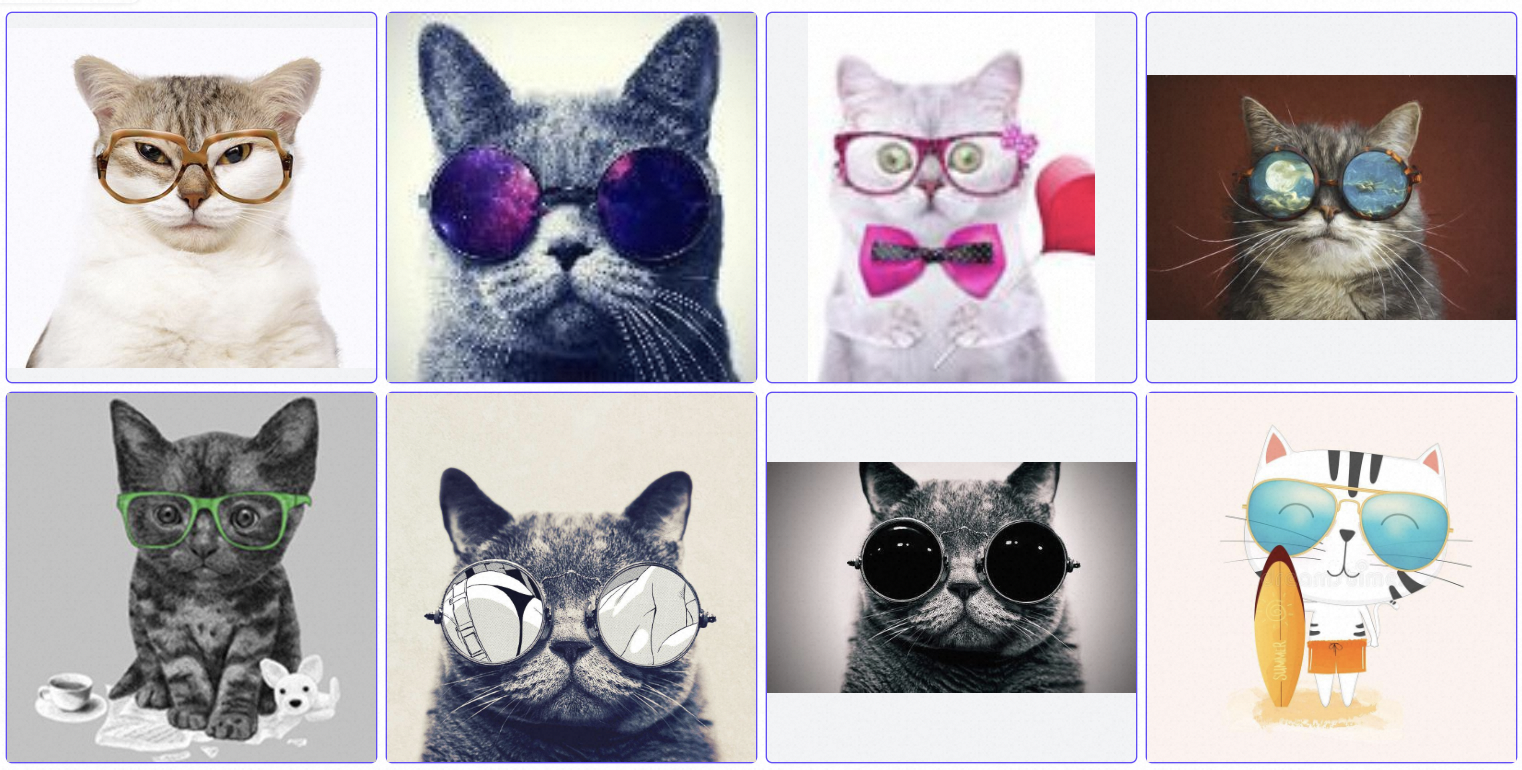
\includegraphics[width=1.0\linewidth]{pics/cat.png}
    \caption{Retrieval results of the query ``a cat with glasses'' in Chinese.}
    \label{fig:demo_cat}
\end{figure*}

\begin{figure*}[h] 
    \centering
    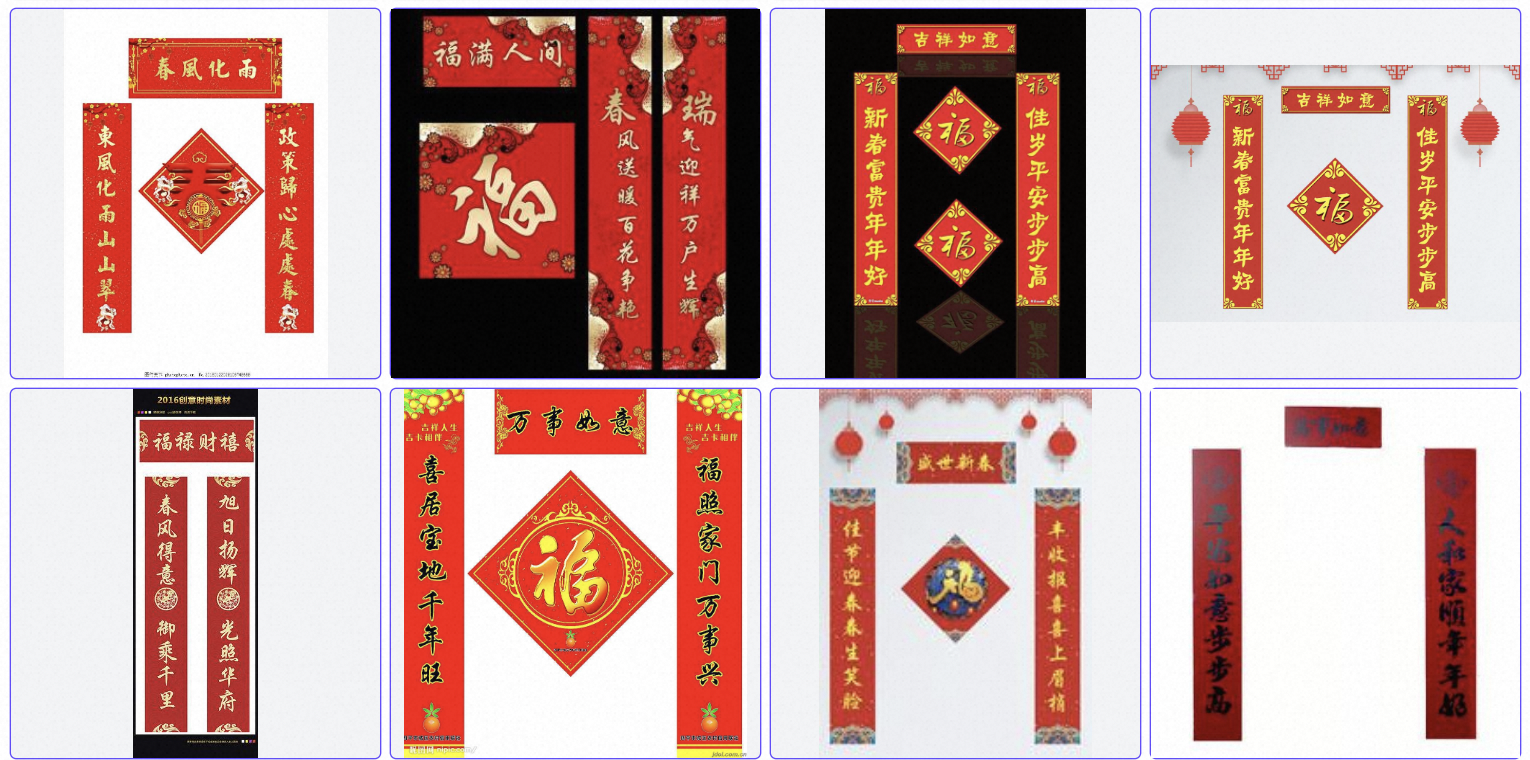
\includegraphics[width=1.0\linewidth]{pics/couplet.png}
    \caption{Retrieval results of the query ``Spring Festival couplet'' in Chinese.}
    \label{fig:demo_couplet}
\end{figure*}

\end{document}
